\documentclass[12pt]{article}
\usepackage[utf8]{inputenc}

\usepackage{graphicx}
\usepackage[T1]{fontenc} 
\usepackage{geometry}

\usepackage{etoolbox}
\usepackage{todonotes}

\usepackage{graphicx}
\usepackage{url}
\usepackage{listings}

\usepackage[ruled,lined]{algorithm2e}

\usepackage[font=footnotesize,labelfont=bf,singlelinecheck=false,center]{caption}

\renewcommand{\baselinestretch}{1,2} 

\bibliographystyle{alpha}

\newcounter{besoin}

% Descriptif des besoins:
% 1 - Label du besoin pour 
% 2 - Titre du besoin
% 3 - Description
% 4 - Gestion d'erreurs
% 5 - Spécifications tests
\newcommand{\besoin}[5]{%
  \refstepcounter{besoin}% 
    \hspace{\stretch{1}} \rule{0.8\linewidth}{1mm} \hspace{\stretch{1}}
    \medskip 
    \begin{center}\label{besoin:#1}\textbf{Besoin~\thebesoin: #2}\end{center}
    \ifstrempty{#3}{}{\textbf{Description:} #3\par}
    \ifstrempty{#4}{}{\textbf{Gestion d'erreurs:} #4\par}
    \ifstrempty{#5}{}{\textbf{Tests:} #5\par}
    \bigskip \bigskip 
    \hspace{\stretch{1}} \rule{0.8\linewidth}{1mm} \hspace{\stretch{1}}
    \bigskip \bigskip 
  }


\newcommand{\besointmp}[5]{%
  \refstepcounter{besoin}% 
    \hspace{\stretch{1}} \rule{0.8\linewidth}{1mm} \hspace{\stretch{1}}
    \medskip 
    \begin{center}\label{besoin:#1}\textbf{Besoin~\thebesoin: #2}\end{center}
    \ifstrempty{#3}{}{\textbf{Description:} #3\par}
    \ifstrempty{#4}{}{\textbf{Gestion d'erreurs:} #4\par}
    \ifstrempty{#5}{}{\textbf{Tests:} #5\par}
  }


\newcommand\tab[1][1cm]{\hspace*{#1}}

\newcommand{\refBesoin}[1]{%
  Besoin~\ref{besoin:#1}%
}

\geometry{hmargin=2 cm}
\geometry{vmargin=2 cm}

\usepackage[hidelinks]{hyperref}
\hypersetup{hidelinks}

\urlstyle{same}


\begin{document}

% end-pageTitle
\begin{center}


\includegraphics[width=0.8\textwidth]{images/logo.jpg}~\\[0.cm]

\textsc{\LARGE Université de Bordeaux}\\[1.5cm]

%\textsc{\Large }\\[0.5cm]

% Title

\noindent\rule{\textwidth}{3pt}
\\
{\huge \bfseries Génération de villes: \\ Analyse des besoins \\ [0.4cm] }
\noindent\rule{\textwidth}{3pt}



% Author and supervisor
\bigskip
\textbf{ \Large SOULAMI}  \Large Mehdi \\
\textbf{ \Large BOUCHET }  \Large Ines \\
\textbf{ \Large EL-KERZAZI }  \Large Mohammed-amine \\
\textbf{ \Large YANG }  \Large Yi \\
\textbf{ \Large NOUAMANI }  \Large Ayoub \\
\vfill
% Bottom of the page
{\large \today}
\end{center}
% end-pageTitle

\newpage

\tableofcontents

\newpage

\section{Résumé}

Dans notre projet nous allons chercher à modéliser une ville en 3D grâce à l'outil Unity, le but de notre création sera de :
\begin{itemize}
	\item Créer un terrain en relief avec une surface plus plane pour placer la ville
	\item Créer une ville entourée d'une muraille pour obtenir un aspect de ville ancienne, ou de ville médiévale
	\item La ville devra être composé de bâtiments le long des routes et à l'intérieur de la muraille
	\item On doit donc aussi y retrouver des routes qui pour les principales sortiront de la ville par des portes situées sur la muraille
	\item Dans la partie extérieure de la ville on doit pouvoir voir aussi des rivières
	\item La création de la ville doit pouvoir être manipulable par une interface pour établir la taille de la ville ou le nombre de bâtiments.
\end{itemize}

\section{Introduction}

Le projet de génération de villes aléatoires consiste à créer une carte d’une ville à partir d'un plan vide, modélisant ainsi les routes, les bâtiments, et d’autres infrastructures, sur une carte
ayant des spécificités environnementales, elles-mêmes générées par le programme.
Pour mettre à bien notre projet, nous allons utiliser des ressources tel que :

\tab - L’article de CityGen et La thèse de George Kelly sur la génération de villes aléatoires

\tab - L’application Toy Town de Watabou
\subsection{Les objectifs}
\begin{itemize}
    
  \item Génération d'un terrain 3D possédant des collines, montagnes, rivières, lacs.
  \item Création de routes principales qui connectent la ville à l'extérieur des murailles, avec des petites routes annexes au sein de la ville et à l'extérieur.
  \item Les routes s'adaptent au terrain, elle doivent être le plus possible sur des surfaces planes.
  \item Une muraille entoure la ville avec des portes dans des endroits stratégiques.
  \item Des places, jardins (au milieu de la ville préférablement).
  \item Plusieurs types de bâtiments : château, ferme, hôtel de ville, mairie, école, qui sont générés grâce a l'algorithme de placement de structures clés, vers le centre de la ville.
  \item On peut avoir des cellules entre les routes où poser des bâtiments, les cellules peuvent être de plusieurs formes, d'un triangle (3 côtés) à un hexagone (6 côtés).
\end{itemize}

\subsection{Les utilisations}

L’utilisation d’un générateur de villes pourrait être utile pour les entreprises cherchant à créer de nouvelles infrastructures dans des villes déjà existantes, ou pour modéliser par exemple des routes sur une carte générée par le programme.

La génération d'une ville médiévale pourrait être utile aux chercheurs dans le domaine historique cherchant à créer une représentation d'une ville ancienne.

Créer des villes est également très utile dans le domaine des jeux vidéos pour modéliser les maps des jeux.

\section{Analyse de l'existant}
\subsection{Citygen}
\subsubsection{Interface et options}

L’interface est simple et facile d’usage, c'est un point and click similaire à un éditeur 3D, il y a trois modes d'édition principaux avec des options d'ajouts et de suppressions : nœuds, routes et cellules. Tout d’abord on peut créer une ville avec un affichage en temps réel avec des routes principales, en rajoutant des noeuds permettant de délimiter les périmètres d'une ville. Une fois ces noeuds reliés avec des arêtes, une cellule de ville est créer, l'affichage de bâtiments ainsi que celui des routes secondaires est automatiquement généré suite à un calcul par le système à l'aide des processus d'échantillonnage, de traçage et d'interpolation pour construire les itinéraires routiers réels à travers le terrain.\\
Les bâtiments ainsi que les routes secondaires s'adaptent donc aux changements appliqués aux routes principales.\cite{KellyLog} \\

La génération d'une ville avec Citygen représente bien la géométrie urbaine typique d'une ville moderne. Avec les options d’affichage ciblé integré, il est plus facile de voir le fonctionnement à travers les tests unitaires effectués.\\

Il existe aussi une vidéo d'utilisation démonstrative sur le site officiel du programme.\cite{video}

\subsubsection{Analyse des options et tests}

Le terrain est une image en .png ayant une perspective en 3D, on peut changer le terrain en y important notre propre image de terrain.

\begin{center}
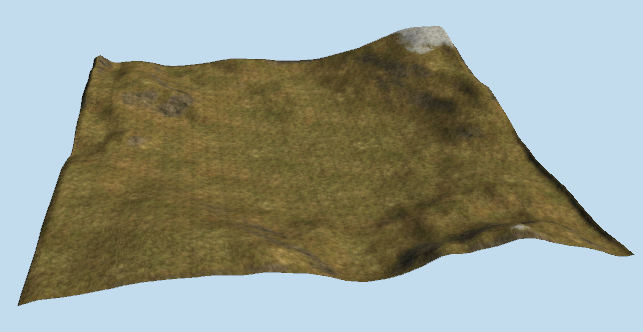
\includegraphics[height = 5 cm]{images/terrain.png}\\
\captionof{figure}{\small{Capture d'écran du terrain 3D du logiciel de base}}

\end{center}

\subsubsection{\textbf{Génération d'une route principale}}

En utilisant le bouton Node Edit puis Add Node, on délimite notre ville en posant 5 noeuds.

\begin{figure} 
\begin{minipage}[c]{.46\linewidth}
	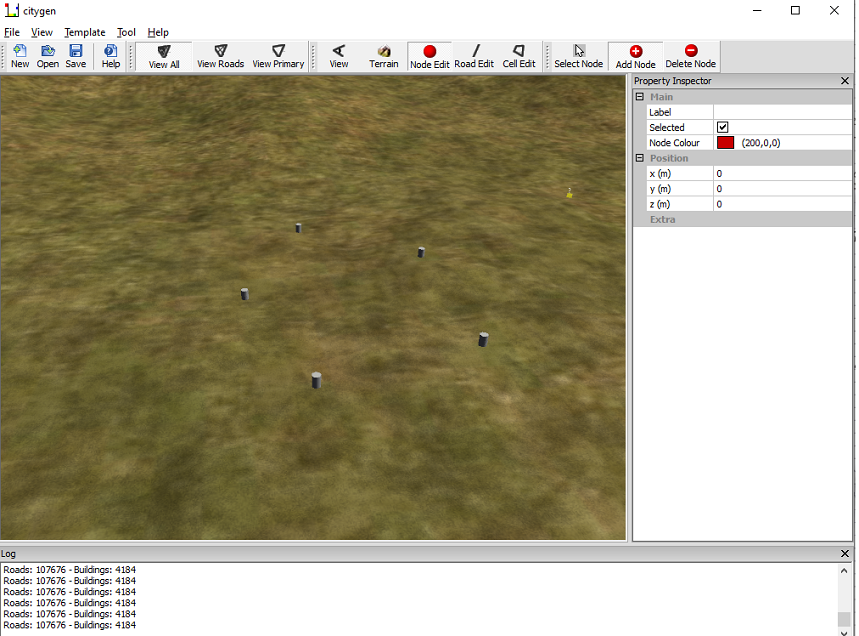
\includegraphics[height = 5 cm]{images/figure1.png}\\
	\captionof{figure}{\small{Capture d'écran personnelle du logiciel Citygen}}
\end{minipage} \hfill 
\begin{minipage}[c]{.46\linewidth}
	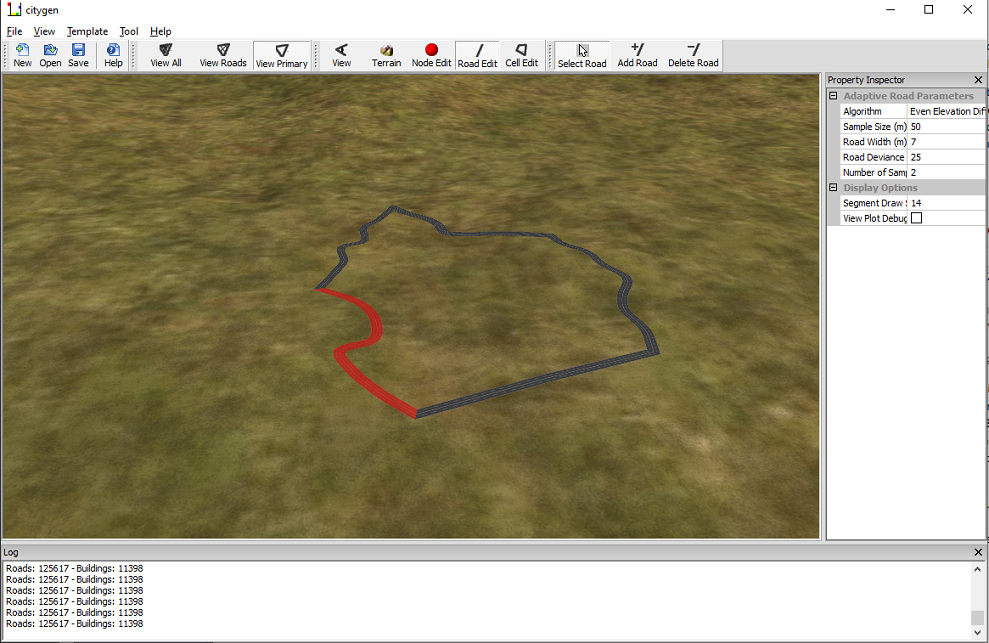
\includegraphics[height = 5 cm]{images/figure2.png}\\
	\captionof{figure}{\small{Capture d'écran personnelle du logiciel Citygen}}
\end{minipage}
\end{figure}

Une fois les noeuds reliés entre eux avec des arêtes, la cellule de ville est créée, on aperçoit la génération de nos routes principales avec des options à droite permettant aux routes principales d'être manipulées de manière interactive.

\subsubsection{\textbf{Génération d'une route secondaire}}

\begin{center}
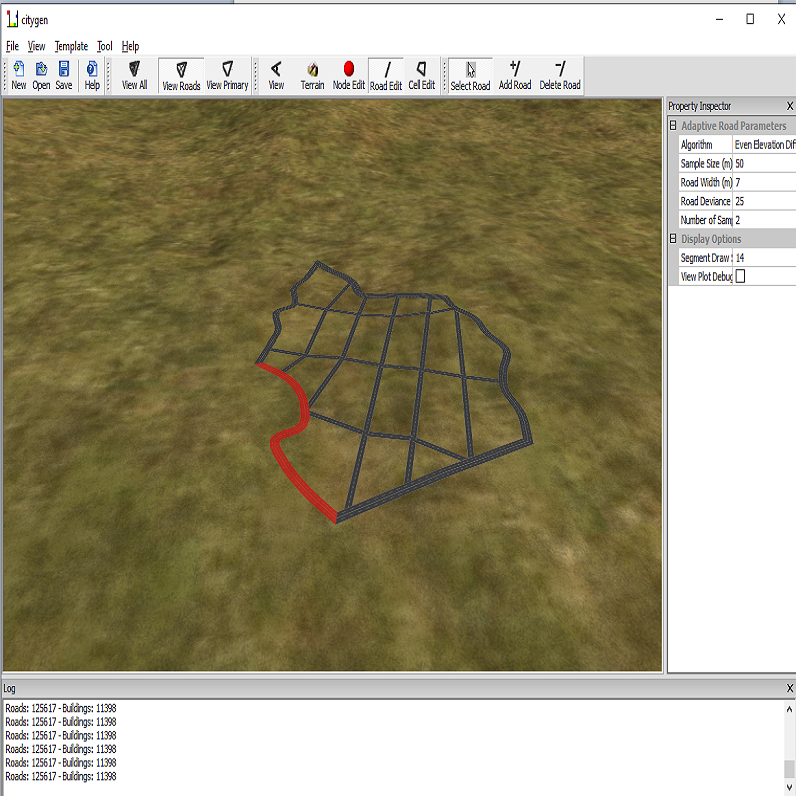
\includegraphics[height = 5 cm]{images/figure3.png}\\
\captionof{figure}{\small{Capture d'écran personnelle du logiciel Citygen}}
\end{center}
Les routes secondaires ne sont modifiables qu'en manipulant les routes principales et sont générées automatiquement à l'aide d'un algorithme basé sur la croissance.

\subsubsection{\textbf{Génération d'un bâtiment}}

Les bâtiments sont générés automatiquement grâce à un processus de lôtissements et sont également modifiables en manipulant les routes principales.
Il y a 125617 routes et 11398 bâtiments.
\newline
On peut aussi ouvrir un fichier de ville moderne (.cgx) conçu et sauvegarder le notre.

\textbf{\tab Entree : } Un fichier de ville (format .cgx)

\textbf{\tab Sortie : } Une représentation graphique d'une ville générée par le fichier
    
    
    \tab Le logiciel vérifie que le fichier d'entrée est un fichier .cgx, il y a 7383 routes et 67759 bâtiments et l'affichage est quasi-instantané.

\begin{figure} 
\begin{minipage}[c]{.46\linewidth}
	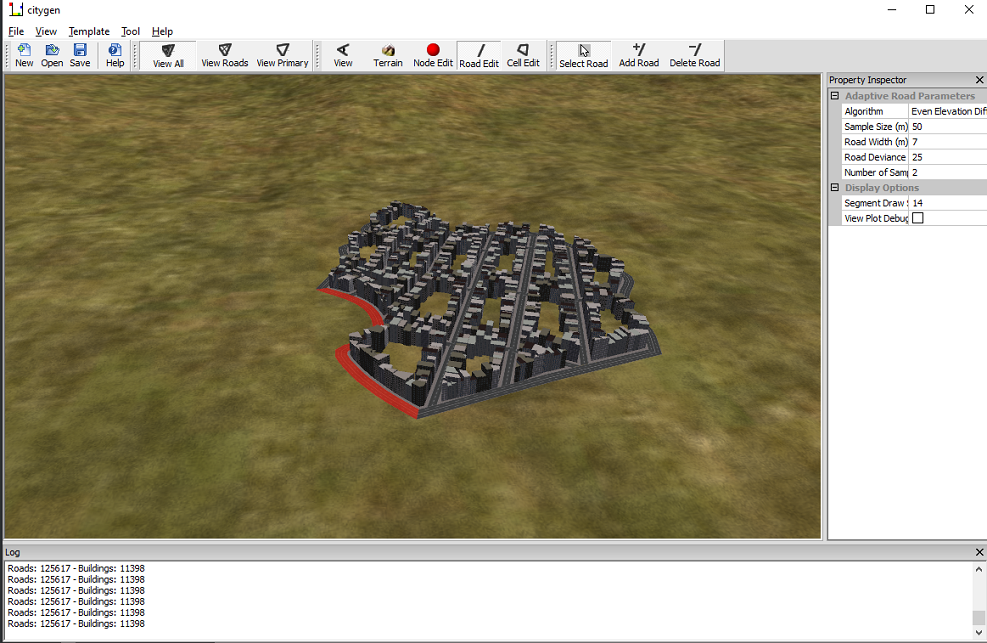
\includegraphics[height = 5 cm]{images/figure4.png}\\
	\captionof{figure}{\small{Capture d'écran personnelle du logiciel Citygen}}
\end{minipage} \hfill 
\begin{minipage}[c]{.46\linewidth}
	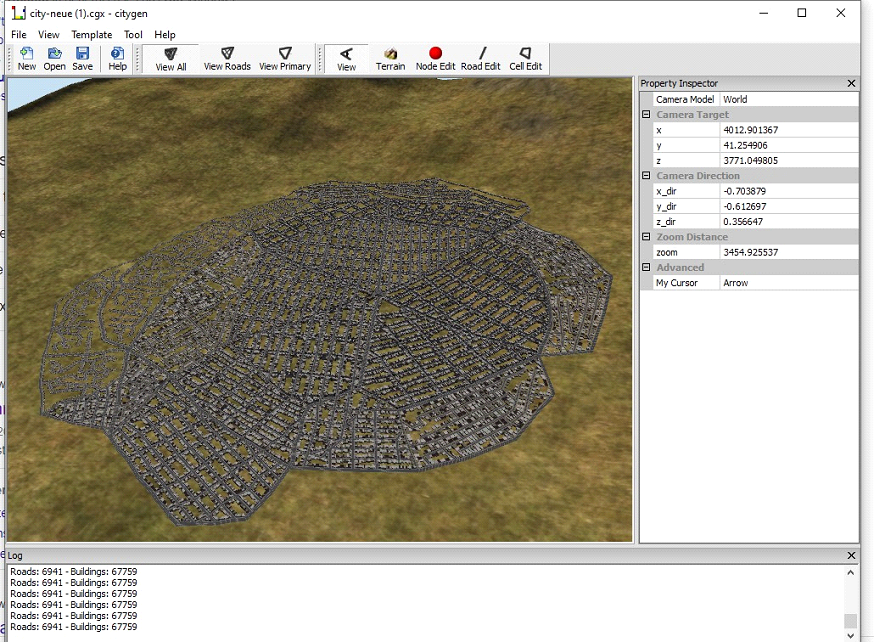
\includegraphics[height = 5 cm]{images/figure5.png}\\
	\captionof{figure}{\small{Capture d'écran personnelle de l'importation d'une ville déjà conçue}}
\end{minipage}
\end{figure}

\subsubsection{Analyse des éléments de la ville}

\subsubsection{\textbf{Les routes principales}}

\begin{center}
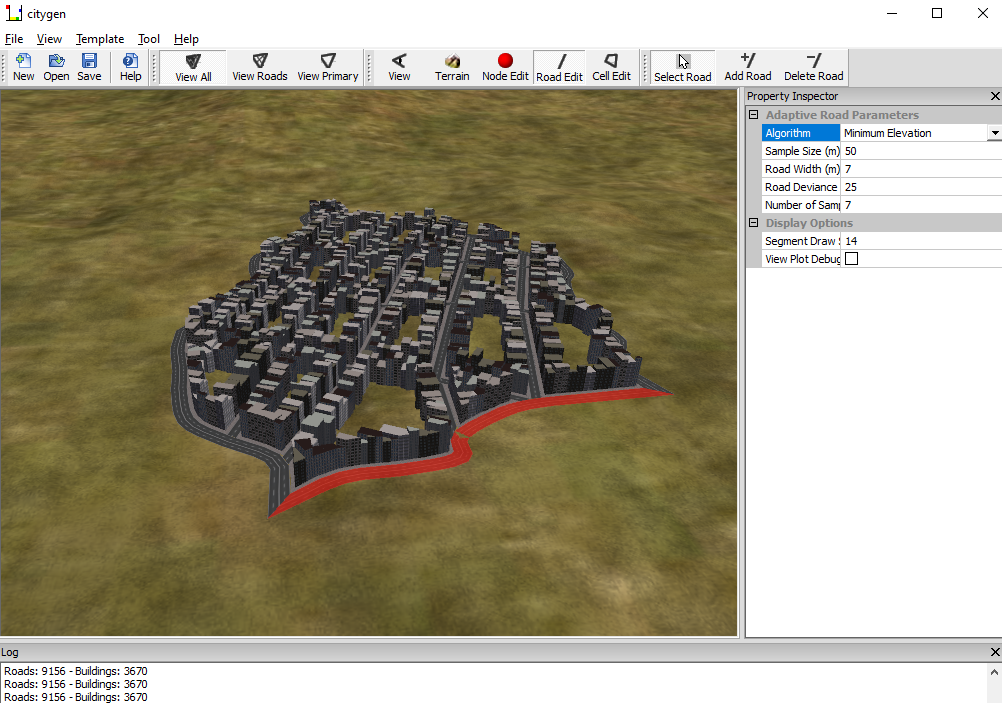
\includegraphics[height = 5 cm]{images/figure6.png}\\
\captionof{figure}{\small{Capture d'écran personnelle d'une route sélectionnée avec l'algorithme Minimum Elevation}}
\end{center}
Route avec l'algorithme Minimum Elevation :
L'échantillon avec l'altitude (Elevation) la plus basse est sélectionnée.

\subsubsection{\textbf{Les routes secondaires}}

\begin{center}
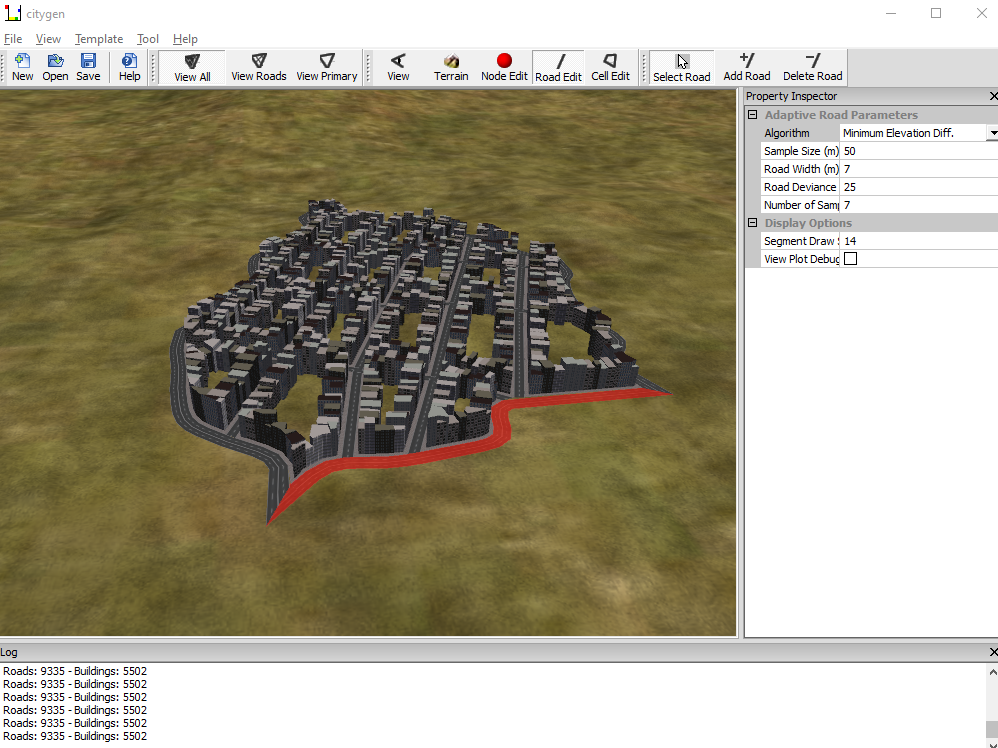
\includegraphics[height = 5 cm]{images/figure6bis1.png}\\
\captionof{figure}{\small{Capture d'écran personnelle d'une route sélectionnée avec l'algorithme Minimum Elevation Diff}}
\end{center}
Route avec l'algorithme Minimum Elevation Diff :
L'échantillon avec une altitude uniforme pour l'ensemble du segment de route.

\subsubsection{\textbf{Les bâtiments}}

\begin{center}
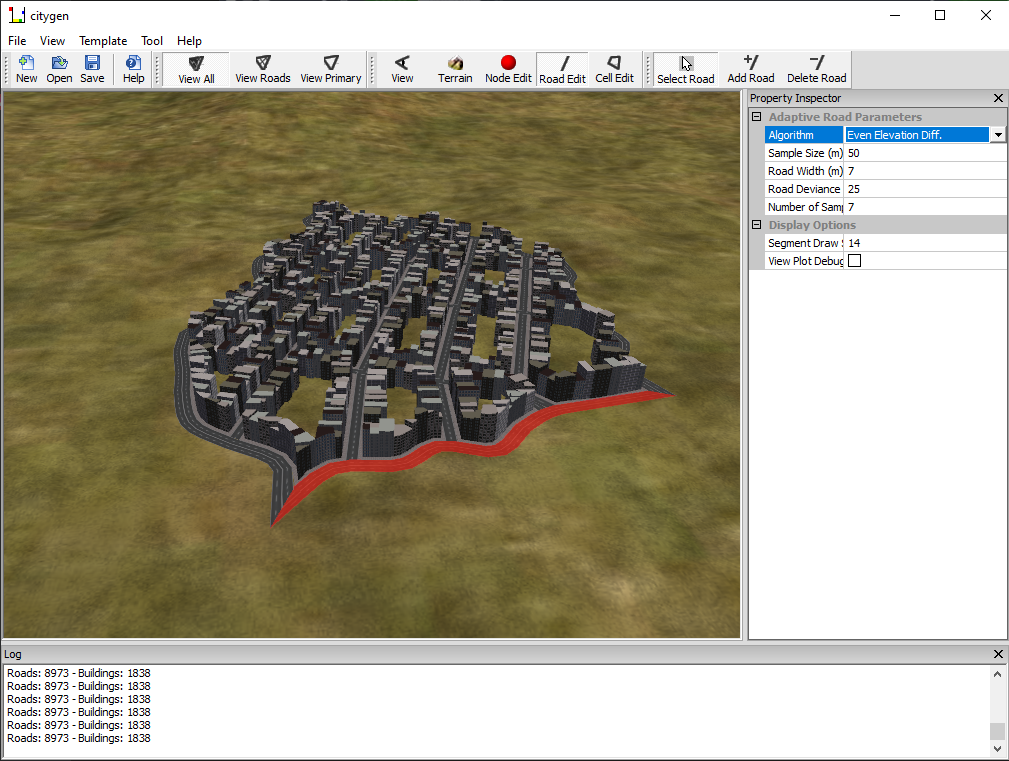
\includegraphics[height = 5 cm]{images/figure6bis2.png}\\
\captionof{figure}{\small{Capture d'écran personnelle d'une route sélectionnée avec l'algorithme Even Elevation Diff}}
\end{center}
Route avec l'algorithme Even Elevation Diff :
L'échantillon avec une altitude uniforme et plus lisse avec plus de courbes.
Le choix de routes selon une altitude est une bonne idée pour une meilleure impression d'une visualisation en 3D.

\subsubsection{Performances de Citygen}
Le logiciel crash de temps en temps quand on essaye de mettre des grandes valeurs en paramètres. Quant au temps d’affichage quand on load un fichier de carte est quasi-instantané, pareil pour la génération de routes.
\subsubsection{Compatibilite}
Le logiciel Citygen ne marche que sur Windows, une carte de ville déjà prête y est fournie pour un test initial.

\subsection{Medieval Fantasy City Generator}
\subsubsection{Interface et fonctionnement}
L'interface est également simple et facile d'usage, un point and click qui inclue, en revanche on a des raccourcis claviers pour les différentes options, le programme nous donne un résultat en 2D sous la forme d'une image où il y a plusieurs éléments de ville de style médievale , comme des citadelles, des temples, des châteaux, des bidonvilles, des fermes, une côte maritime, des rivières, des zones vertes (forêts, etc...), des routes, des murs, des arbres.. Il est possible de changer la couleur des écritures et l'ensemble des éléments de la carte grâce à un code de couleur en héxadécimal ou une configuration manuelle en HSV.

\subsubsection{Analyse des options et tests}

Il y a également plusieurs options proposées comme la génération d'une nouvelle ville aléatoire avec un nom aléatoire et des noms de districts qu'on peut ensuite modifier, soit en cliquant sur le texte directement ou bien à travers l'option Settlement, on peut également ajouter un nouveau texte directement avec l'option Landmark.\\

Il y a l'outil Warp permettant de manipuler les différentes options de générations, comme celle qui permet de modifier la taille des routes ainsi que les batîments, ajouter de l'eau, égaliser les éléments affichés, mesurer, déplacer, appliquer une rotation à la ville, il y a également une option interessante qui permet de défaire les modifications qu'on souhaite appliquées et qui n'ont pas été appliquées encore.\\

On a la possibilité d'enregistrer notre ville générée sous la forme d'une image en PNG, mais également de générer une ville sur mesure mais d'une manière aléatoire en choississant les éléments de ville possibles qu'on y souhaite intégrer, ainsi que le nombre de routes (un nombre par défaut, maximal ou bien encore pré-défini), et la taille de la ville souhaîtée (Small, Medium, Large).\\

On peut également enregistrer ou bien partager la ville générée à travers un lien permanent qu'on peut avoir sous forme d'URL, ou encore bien sous la forme d'un fichier SVG pour une perte minimale de la qualité d'image. Il y a la possibilté d'enregistrer sous la forme d'un fichier JSON pour les changements de style et de couleurs.\\

Le partage sous forme d'URL fonctionne correctement, conserve les proportions ainsi que les noms donnés, mais ne conserve pas les modifications de styles, les différentes couleurs des éléments de la ville, la taille, la police et le style des noms de villes.\\

Pour l'exportation du style il faut avoir recours au fichier JSON, mais l'import d'un fichier de style JSON ne semble pas fonctionner.
Il y a aussi une échelle représentant la distance sur la carte et sa correspondance sur le terrain, tandis que la boussole est purement  décorative (ne change pas dans le cas d'une rotation).
Il y a également une option pour un affichage plein écran \cite{medieval}
\begin{center}
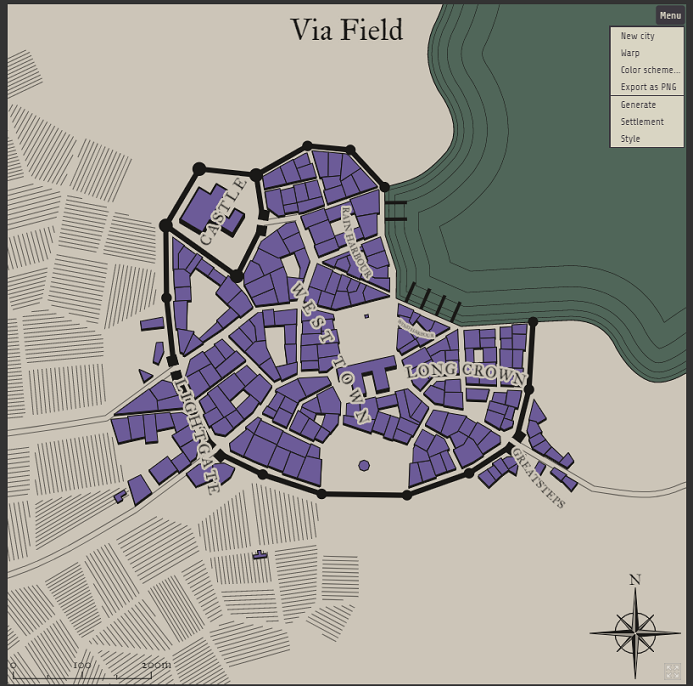
\includegraphics[height = 5 cm]{images/figure8.png}\\
\captionof{figure}{\small{Capture d'écran prise sur une machine personnelle d'une ville générée avec le programme}}
\end{center}

\subsubsection{Performances de Medieval Fantasy City Generator}

Le programme web prends un temps de moins d'une seconde quand il s'agit de générer une ville aléatoirement ou bien avec des choix pré-définis, et une à deux secondes quand il s'agit d'appliquer des modifications sur les éléments de la ville.

\subsubsection{Compatibilité}

Le programme est compatible avec la majorité des appareils nouvelles générations et donc l'ensemble des systèmes d'exploitations supportant un navigateur Web capable d'afficher du JavaScript (iOs, Android,
MacOS, GNU/Linux, Windows ...).

\subsubsection{Performances de la machine de test}

\begin{center}
  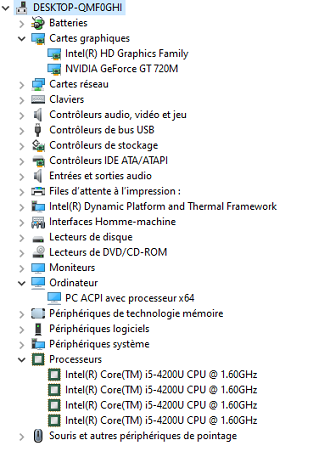
\includegraphics[height = 7 cm]{images/figure9.png}
  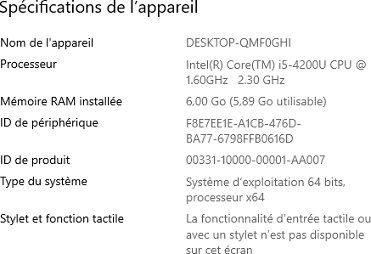
\includegraphics[height = 7 cm]{images/figure10.png}\\
  \captionof{figure}{\small{Specification de l'appareil}}
\end{center}

Ces tests et ces captures de logiciels ont été réalisées sur une machine personnelle dôtée d'un processeur x64 i5 à deux coeurs, 1.60GhZ 2.30 GHz, une Ram de 6 Go et une carte graphique NVIDIA GeForce GT 720M, une configuration plutôt moyenne qui permet de faire marcher ces logiciels existants avec de bonnes performances.

L'accessibilité ainsi que la faisabilité du projet sur une machine moyenne montre que le projet est à la fois à portée de beaucoup de monde, mais aussi réalisable d'un côté developpement.


\newpage

\section{Besoins non-fonctionnels}

\subsection{Systeme de priorité}

\begin{center}
\colorbox{red}{\color{red}CouleurcouleurCouleurcouleur}\\ Couleur rouge : Priorité élevée \\

\bigskip

\colorbox{cyan}{\color{cyan}CouleurcouleurCouleurcouleur}\\ Couleur verte : Priorité moyenne\\

\bigskip

\colorbox{brown}{\color{brown}CouleurcouleurCouleurcouleur}\\ Couleur noire : Priorité faible 
\end{center}
 
\besoin{}
{\textcolor{cyan}{Taille de la ville }}
{ 
\begin{itemize}
  \item Une ville qui en plus de l'infrastructure (places, jardins, chateau, marche, fermes, hôtels de ville, mairie, église, écoles), également un certain nombre de bâtiments résidentiels afin que le nombre de bâtiments dans la ville soit au moins supérieur à 100.
 \item Le nombre total de bâtiments dans la ville est inférieur à 10 000,  ce qui est bien moins que le nombre de citadins, mais la taille de la ville est limitée par le fait qu'elle a été construite au Médiéval .
 
 \item Ce nombre peut être augmenté en fonction des performances des algorithmes .
 
\end{itemize}
}
{}
{}
\besoin{}
{\textcolor{cyan}{Temps de génération}}
{le temps de génération du plan  doit être raisonnable. Grâce aux algorithmes impliqués, Le modèle de la ville (Citygen) présenté contient plus de 24 000 bâtiments et le temps de génération complet de la ville, y compris les routes adaptatives, les routes secondaires et les bâtiments, n'est que de 3,5 secondes.

Les bâtiments sont actuellement texturés en utilisant seulement un petit nombre de matériaux.
}
{}
{
\begin{itemize}
 \item\textbf{ Description : } Vérifier que le temps de génération une ville avec une taille entre intervalle (1000, 10000)  est inférieur à 5 secondes.  \\
 \textbf{Entrée : } un modèle de ville avec 5000 baîments.  \\
 \textbf{Sortie Attendu : } Le temps de génération soit inférieur à 5 secondes . \\
 \textbf{Déroulement du test: } On crée un compteur pour calculer le temps qu’il dépense après chaque lancement de chaque Génération test. 
 
 \item\textbf{ Description : }  Vérifier qu'une ville en taille plus grande que la limite est non acceptée par le générateur de ville.  \\
 \textbf{Entrée : }  un modèle de ville avec 50000 batîments (hors de la taille acceptée).  \\
 \textbf{Sortie Attendu: } Affiche une indication que la plage acceptable a été dépassée. 
\end{itemize}
}
\besoin{}
{\textcolor{red}{Interface}}
{
Le programme doit intégrer une interface utilisable par le client, possédant des boutons spécifiques (voir besoin Fonctonnalités de l'interface) et un aspect clair et fonctionnel.

\begin{itemize}
\item L’utilisation d’un symbole largement compris (comme une poubelle pour un bouton de suppression, un signe plus pour ajouter quelque chose, ou une loupe pour la recherche) en combinaison avec du contenu.

\item Choisir une couleur avec une signification pertinente (vert pour un bouton « commencer à générer », rouge pour « arrêter de la génération»).

\item Surligner le bouton correspondant à l’action souhaitée.

\item Pour les actions ayant des conséquences irréversibles, comme la suppression permanente de fichier. On  demande aux utilisateurs s’ils sont sûrs de vouloir passer à l’action.
\end{itemize}
}
{}
{
\begin{itemize}

\item \textbf{Description : } Vérifier que les symboles de bouton correspondent à leur action.\newline
\textbf{ Analyse du test: } Tester le signification des boutons utilisables sur l'interface. \newline


\item \textbf{ Description : }Vérifier que le programme affiche une indication waring quand l'utilisateur souhaite exécuter une action  irréversibles. \newline
\textbf{Déroulement du test : } On demande de supprimer le plan courant  \newline
\textbf{Entrée : } Un programme générant une interface pour l'utilisateur.\newline
\textbf{Sortie Attendu : }  L'affichage d'une indication waring.

\item \textbf{ Description  : } Vérifier que  tous les boutons ont été surligné quand l'utilisateur choisi une action.
\textbf{Déroulement du test : } On clique tous les actions proposées et voir s’ils ont été surlignées. \newline
\end{itemize}
}
\besoin{}
{\textcolor{cyan}{Possibilité de récupération} }
{ 
A partir du deuxième évolution de ville , L’utilisateur peut récupérer une version anciennes de ville. Après chaque évolution, nous stockons les nouvelles pièces dans un tableau dans l'ordre, le numéro de série correspondant est sa version, et chaque fois que nous revenons à la version précédente, nous montrons simplement les nouvelles pièces qui ont été ajoutées.
}
{}
{
\begin{itemize}
 \item  \textbf{ Description: } Vérifier que tous les versions anciennes de villes peuvent être récupérées.\\
 \textbf{ Entrée : } des numéro de l’anciennes versions . \\
 \textbf{Sortie Attendu : } Une représentation graphique d’une ville en version ancienne demandée. \\
 \textbf{Déroulement du test: } Effectuer une géneration de ville et choisir une version de ville ancienne.  
 
 \item \textbf{ Description: } Vérifier qu'une demande de version non-existante ne bloque pas le système. \\
 \textbf{Entrée : } un numéro de la version ville non-existante. \\
 \textbf{ Sortie Attendu: } Affiche un message d'erreur. 
\end{itemize}
}
\besoin{} 
{\textcolor{cyan}{Pente de la route }}
{
Le calcul du pourcentage de la pente du terrain permet de connaître le type de pente : pente douce, modérée ou forte. 

     - route pente forte est 8 \%-12 \% 

     - route pente modérée est 5 \%-8 \%

     - route pente douce est 0 \%-5 \%

Le calcul de la pente est exprimé en pourcentage et s’obtient en appliquant la formule suivante : \\

Pente (\%) = Dénivelé (m) / Longueur parcourue (m) \\

Dénivelé = Hauteur totale entre le point d'arrivée et le point de départ.
}
{}
{}

\newpage

\section{Besoins fonctionnels}

\besoin{}
{\textcolor{red}{Générer un terrain}}
{
Le programme doit créer un terrain. Optionnellement, on ajoutera des éléments environnementaux (Besoin 9). \\
Le terrain correspond à une surface en relief, représenté en deux dimensions, de forme carrée ou rectangulaire, dans lequel on pourra exploiter sa surface pour générer des éléments environnementaux, des bâtiments et des routes.
La création du terrain devra avoir l'objectif de permettre de créer une ville médievale sans avoir d'inconveniant geographique, c'est-à-dire, l'emplacement pour la ville sera amenagée suivant les contraintes suivantes:

\begin{enumerate}
\item Emplacement loin des montagnes et collines pour éviter des innondations et encerclement facile des adversaires en cas de guerre.
\item Proche de toute source d'eau (rivière, lac ou mer/ocean).
\item Entourée de terrains fertiles à l'agriculture.
\item Zone principalement plane.
\end{enumerate}
 Les éléments environnementaux seront ajoutés en respectant la géographie (ex: arbre ayant sa base en contact avec la surface du terrain).
}
{}
{
\begin{enumerate}
\item \textbf{\tab Description : } Vérifier que le terrain créé (valeurs dans le tableau généré) ne contient pas des valeurs aléatoires.\\

\textbf{\tab Déroulement du test : } En utilisant le bruit de Perlin avec les mêmes valeurs utilisées pour produire le premier fichier, on obtiendra un deuxième fichier. Ce fichier sera utilisé pour comparer les deux  tableaux.\\
\textbf{\tab Entrée : } Un tableau [longueur, largeur] contenant une valeur z (hauteur) pour chaque case. 
\end{enumerate}
  
}
\newpage
\besoin{}
{\textcolor{red}{Génération du réseau routier principale}}
{Le programme prend en entrée un terrain pour y créer un réseau de routes conformes et logiques. "Une route principale est une route reliant deux pôles agglomérés de niveau départemental ou régional, supportant un trafic important non strictement local, évitant parfois les traversées d'agglomération. On utilise en milieu urbain plutôt le terme « artère principale »". On doit au maximum éviter les impasses, c'est-à-dire, on essaiera d'avoir chaque noeud (rond point ou croisement) possédant au moins deux arêtes adjacentes (routes) qui menent vers des autres noeuds. \cite{routePrincipale} De plus, la distance entre les deux doit être suffisamment éloignée pour ne pas créer un système de routes trop complexe.
\begin{center}
    \centering
    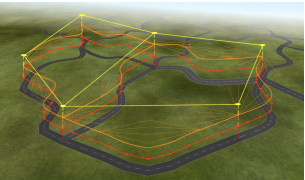
\includegraphics[height = 3 cm]{images/route_principale.png}\\
    \captionof{figure}{\small{Exemple de représentation d'un route principale reliant dans un terrain.}}
\end{center}
}
{}
{
    \begin{enumerate}
    \item \textbf{\tab Description : } Vérifier que les routes principales sont connectées entre-elles.  \\
    \textbf{\tab Déroulement du test : }  Détecter si les noeuds représentants des croisements sur les routes principales soient au moins connectées à deux arêtes, et que cette connexion entre chaques noeuds représente un graphe connexe.\\
    \textbf{\tab Entrée : } une liste chaînée avec les nœuds et les nœuds adjacents. Cette liste est la représentation des routes créées dans notre plan. \\
    
    \textbf{\tab Description : } La distance entre chaque nœud doit être au moins X distance .\\  
    \textbf{\tab Déroulement du test : }  Programme qui calcule la distance entre deux nœuds.\\
    \textbf{\tab Entrée : } une liste chaînée avec les nœuds et les nœuds adjacents. Cette liste est la représentation des routes créées dans notre plan. \\

  \end{enumerate}
}

\newpage

\besoin{}
    {\textcolor{red}{Génération des routes secondaires}}
    { Le programme doit pouvoir créer les routes secondaires dans un terrain avec les routes principales créés. \\
    Définition de routes secondaires : "Les termes “routes secondaires” concernent généralement l’ensemble des voies de circulation aménagées dans un environnement rural, et dont la vocation première est de permettre une circulation fluide des usagers vivant près de ces voies spécifiques, et devant circuler sur de faibles distances. Ces voies s’éloignent alors des routes principales, qui ont un rayonnement au niveau national ou niveau local, sur une étendue dépassant une simple zone locale grâce à la structuration du réseau routier local que ces routes principales apportent." \cite{routeSecondaire}
    \begin{center}
        \centering
        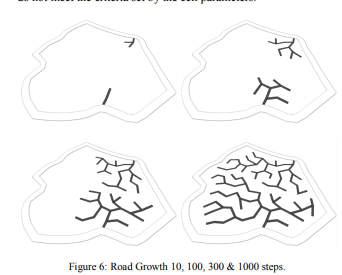
\includegraphics[height = 5 cm]{images/routes_secondaires.png}\\
        \captionof{figure}{\small{Exemple de représentation d'un route secondaires dans une ville.}}
    \end{center}
    }
{}
{ 
    \begin{enumerate}
    \item \textbf{Description : } Détecter si tous les nœuds ont au moins une route menant vers tous les autres noeuds.\\
    \textbf{Déroulement du test : } On a un programme qui teste chaque nœud vers une liste non NULL, c’est-à-dire, notre graphe ne devra pas contenir un nœud/graphe non connexe (ex: algorithme de Dijkstra). 
    \textbf{Entree : } Le programme prend en entrée un terrain avec un réseau de routes principales pour y créer un réseau de routes secondaires. \\

    \item \textbf{Description : }  Proximité entre les routes.\\
    \textbf{Déroulement du test : } L’algorithme doit vérifier que les routes secondaires sont créées en respectant un périmètre minimum entre deux routes secondaires.\\
    \textbf{Entree : } Le programme prend en entrée un terrain avec un réseau de routes principales pour y créer un réseau de routes secondaires. \\

    \item \textbf{Description : } Vérification que les routes respectent la stratégie dont elles se sont générées.\\
    \textbf{Déroulement du test : } Calcule la moyenne de l’altitude des points échantillonnés et comparer avec la moyenne des points dans un rayon fixe, les contraintes de comparaison sont différentes pour chaques strategies.\\
    \textbf{Entree : } Tableau de points de sortie | Tableau de points pour comparer.\\


  \end{enumerate}
}
\besoin{}
{\textcolor{red}{Normaliser les routes}}
{
Les routes sont créées pour qu'elles soient le plus naturel possible, pour cela on aura des variations entre des routes droites, des routes avec des ondulations qu’on peut contrôler.
Les routes droites ont une marge de bruit ce qui fait qu'elles ne sont pas parfaitement droite.
On a un maximum d’une seule ondulation par génération de route entre deux points pour éviter d’avoir une route fortement sinusoïdale. le côté de l’ondulation va dépendre de l’algorithme utilisé. 
On doit également prendre en compte le terrain utilisé, en effet, on ne peut pas créer une route parfaitement stable sur un emplacement montagneux, si le terrain ne nous permet pas d'avoir une route droite ou ondulée, on utilisera une route qui ne sera pas normalisée. Sur les surfaces planes, les routes devront être les plus droites possibles.

\begin{center}
    \centering
    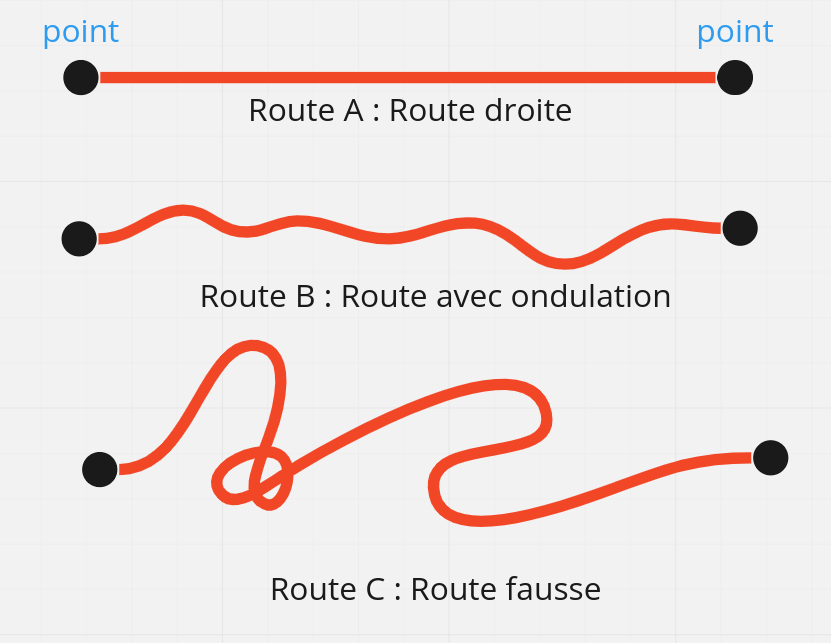
\includegraphics[height = 5 cm]{images/types_de_routes.png}
\end{center}
}
{}
{
\begin{itemize}

\item \textbf{\tab Description : } Vérifier que toutes les routes ne font pas plus d’une ondulation entre deux points.\newline
\textbf{\tab Déroulement du test : } On additionne 0 et 0’ pour chaque point et on compare si la somme respecte la contrainte fixée par le développeur.\newline
\textbf{\tab Entrée : } Tableau de points entre un point source et un point arrivé.\newline
\textbf{\tab Analyse du test : } Utilisation des théorèmes de trigonométrie de base.

\item \textbf{\tab Description : } Vérifier que les points échantillonnés forment une liaison entre le point source et le point de destination.\newline
\textbf{\tab Déroulement du test : } le point de départ doit être à l’indice [0] et le point d’arriver à l'indice du nombre de point dans le tableau - 1.\newline
\textbf{\tab Entrée : } Tableau de points entre un point source et un point arrivé.

\item \textbf{\tab Description : } Vérifier que les points échantillonnés entre le point source et la destination respectent un espacement normalisé.\newline
\textbf{\tab Déroulement du test : } calcule la distance et l’angle 0 entre chaque couple de deux points et les comparer avec les contraintes fixée par le développeur.\newline
\textbf{\tab Entrée : }  Tableau de points entre un point source et un point arrivé.\newline
\textbf{\tab Analyse du test : } Opérations de comparaison.

\end{itemize}
}
\besoin{}
{\textcolor{red}{Générer des cellules entre les routes}}
{
Les cellules urbaines sont formées à partir des régions fermées du réseau routier primaire et secondaire, c’est un espace vide entre des routes qui permettra d'héberger les bâtiments de la ville.\\

Une cellule est composée de 3 côtés minimum c’est à dire que la cellule la moins compliquée est un triangle.\\

La taille d’une cellule doit être régulée entre une valeur maximal et minimal qui évitera d’avoir des cellules très importantes de tailles (irréalistes), ni des cellules ou on peut pas poser des bâtiments. Les petites cellules générées seront supprimées.

\begin{center}
  \centering
  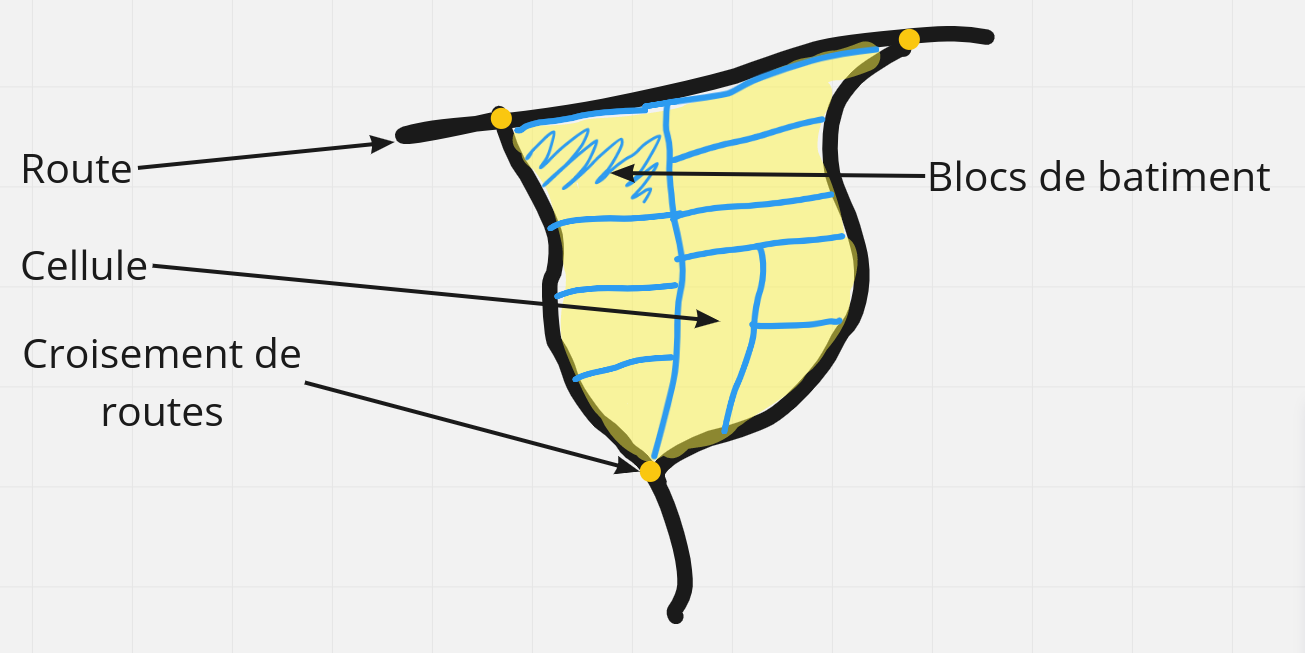
\includegraphics[height = 6 cm]{images/cellule.png}\\
\end{center}

}
{}
{

\begin{itemize}

\item \textbf{\tab Description : } vérifier qu’une cellule est composée de 3 points minimum.\newline
\textbf{\tab Déroulement du test : } Tester qu’une cellule a plus de trois côtés (trois hauteurs).\newline
\textbf{\tab Entrée : } Un tableau de sommets | un tableau d’indices de sommets pour chaque cellule.


\item \textbf{\tab Description : } Vérifier que tout les côtés d’une cellule sont reliés entre eux.\newline
\textbf{\tab Déroulement du test : }  Vérifier qu’il existe une seule instance d’un point sauf pour le point de départ qui doit être le point du début et de la fin.\newline
\textbf{\tab Entrée : } Un tableau de sommets | un tableau d’indices de sommets pour chaque cellule.\newline
\textbf{\tab Analyse du test : }  Algorithme de Martello pour la vérification d’un graphe Hamiltonien, les points du tableau sont représentés comme sommets du graphe et l’ordre des points sera représenté comme arêtes.

\item \textbf{\tab Description : } Vérifier qu'il y a au minimum un nombre de cellules, on peut modifier le nombre minimum qui représente une gestion d’erreur.\newline
\textbf{\tab Déroulement du test : } Calcule de la somme des cellules qui doit être supérieure à une contrainte fixe.\newline
\textbf{\tab Entrée : } tableau d’indice de sommets pour chaque cellule.
\end{itemize}
 }
\besoin{}
{\textcolor{red}{Générer des bâtiments}}
{
Le programme doit pouvoir créer un bâtiment, en affichage 3D, en tenant compte des caractéristiques de la parcelle utilisée, tel que la hauteur du sol ou la présence ou non d'éléments de type lacs ou rivières. Le bâtiment aura un aspect rectangulaire et sa couleur tiendra compte de son type. Son implantation ne peut pas être sur une surface qui n’est pas assez plane pour accueillir un bâtiment avec une base plate.

\begin{itemize}
	\item Une \textbf{maison} : 
		\begin{enumerate}
			\item correspond à un bâtiment créé en 3D,
			\item sa base peut être rectangulaire, carré ou triangulaire
		    \item sa taille ne doit pas être très élevée (Elle ne doit pas dépasser la hauteur d’une résidence ou d’un hôpital par exemple). 
		\end{enumerate}
	\item Un \textbf{immeuble} :
		\begin{enumerate} 
			\item est un bâtiment créé en 3D, 
			\item sa forme doit être rectangulaire, 
			\item sa taille doit être suffisamment élevée (il doit être obligatoirement plus haut qu’une maison, au moins trois fois sa hateur)
		\end{enumerate}
	\item Un \textbf{hôpital} : 
	    \begin{enumerate}
		    \item répond aux mêmes normes qu’un immeuble, 
			\item doit par se situer obligatoirement en centre-ville, pour être accessible facilement par tous les domicile qui l’entoure,
			\item doit être prêt d’une ou plusieurs votre principale
		    \item 	peut se constituer un ou plusieurs bâtiments côte à côte (ex: zone hospitalière).
		\end{enumerate}
	\item Un \textbf{commerce} :
		\begin{enumerate}
			\item a les mêmes caractéristiques qu’un hôpital, 
			\item pas de taille prédéfinie (ex : petit commerce ou grand) 
		\end{enumerate}
	\item Une \textbf{ferme} :
		\begin{enumerate}
			\item a les mêmes caractéristiques qu'une maison
			\item doit être placée en dehors de la ville et vers l'extrémité de son extension (l'évolution de la ville écrase les fermes et les fait réapparaître avec le même algorithme).
		\end{enumerate}
\end{itemize}
}
{}
{
\begin{itemize}

\item \textbf{\tab Description : } Vérification que le fichier d'entrée est un fichier de code de langage valide et conforme, et qu'il ne soit pas corrompu.\newline
\textbf{\tab Déroulement du test : } On lance un compilateur et on voit si l'exécutable nous a été fourni, puis on l'exécute. \newline
\textbf{\tab Entrée : } Un programme de génération de bâtiment. \newline
\textbf{\tab Analyse du test : } Fonctionnement du code.

\item \textbf{\tab Description : }Vérification que le fichier de sortie correspond aux caractéristiques du bâtiment demandé et qu'il ne soit pas corrompu.\newline
\textbf{\tab Déroulement du test : } On crée un bâtiment et on vérifie si il représente bien un bloc 3D de la hauteur correspondante à sa description, que la couleur établie soit respectée.\newline
\textbf{\tab Entrée : } Un programme de génération de bâtiment.

\item \textbf{\tab Description : } Verification que le fichier de sortie soit adéquat aux caractéristiques environnementales du plan utilisé, et vérification du respect de la zone utilisée.\newline
\textbf{\tab Déroulement du test : } On essaie d'ajouter un bâtiment sur un lac ou une montagne et on voit si ça fonctionne ou non, et pour les bâtiments de type hopitaux et commerces, on voit si la zone demandé est respectée (centre ville, grand commerce excentré). \newline
\textbf{\tab Entrée : }  Un programme de génération de bâtiment. \newline
\textbf{\tab Analyse du test : } Respect des normes environnementales.

\end{itemize}
} 
\besoin{}
{\textcolor{cyan}{Positionner les structures clé}}
{
Les structures clé sont des annexes aux bâtiments de base, elles sont positionnés dans des cellules comme les bâtiments et caractérisés par leur forme visuel unique, c'est-à- dire que chaque structure a une forme et un affichage différent des autres.\\

Les structures clé telle que : places, jardins, marches, sont placés dans des endroit adapté à la réalité.\\

Les places et jardins doivent être placés dans des endroits plus au centre de la ville.\\

Le centre ville est un cercle posé aléatoirement vers le milieu de la ville avec un rayon bride.
}
{}
{

\begin{itemize}
   
 \item \textbf{\tab Description : } Vérifier que les structures clés sont situées au centre de la ville.\newline
\textbf{\tab Déroulement du test : } Calcule de la distance entre le centre de ville et de la structure et vérifier qu’elle est inférieur à une valeur prédéfinie.\newline
\textbf{\tab Entrée : } coordonnées des structures clé, coordonnées centre de la ville.
\end{itemize}

}
\besoin{}
{\textcolor{cyan}{Placer des lacs et des rivières}}
{
Le programme doit pouvoir créer des caractéristiques concernant l'environnement de la ville et du terrain, tel que des lacs et des rivères. La représentation de ces éléments doit être en doivent prendre en compte un paramètre de hauteur. 
\begin{itemize}
	\item Une \textbf{rivière} dépend de la gravité, elle doit être établie dans une cavité du plan, donc une zone où la hauteur est inférieur à zéro et ne doit pas dépasser la hauteur des parois établies par sa délimitation. 
	La rivière ne peut pas couler sur une pente montante et une rivière possède toujours une entrée et une sortie, l’entrée se fait soit par une montagne soit par un océan et la sortie toujours en océan.
	La forme de la rivière doit être linéaire avec une entrée et une sortie.
	\item Le \textbf{lac} est un point d'eau sur une cavité du plan avec des bords de même hauteur, pour tous points A et B positionnés sur les bords du lac, la hauteur de A est égal à la hauteur de B sur le même axe. 
	Un lac peut être seul ou à l'issus de l'écoulement d'une une rivière : il est possible qu’une rivière passe son chemin par un lac entre son entrée et sa sortie.
\end{itemize}
}
{}
{
\begin{itemize}

\item \textbf{\tab Description : } Vérification que le fichier de sortie correspond aux caractéristiques de l'objet demandé et tienne compte de la profondeur et de la hauteur, et qu'il ne soit pas corrompu. \newline
\textbf{\tab Déroulement du test : } On lance un programme qui tiens en compte les creux pour y placer les arrivées d'eaux et on voit si elles sont correctement générées. \newline
\textbf{\tab Entrée : } Un programme de génération des éléments environnementaux. \newline
\textbf{\tab Analyse du test : } Fonctionnement de la génération.

\item \textbf{\tab Description : } Vérification des contraintes établies sur les objets : 
    - pas de rivières qui monte une montagne
	- pas de lac qui "déborde" de la hauteur de son périmètre\newline
\textbf{\tab Déroulement du test : } On lance le programme et on voit si on génère correctement un lac ou une rivière en respectant la profondeur5 et la couleur (bleu). \newline
\textbf{\tab Entrée : } Un programme de génération des éléments environnementaux.
\end{itemize}
}
\besoin{}
{\textcolor{brown}{Faire évoluer la ville}}
{
Le programme doit montrer une ville évolutive en fonction d'un paramètre temporel, toujours en tenant compte des caractéristiques environnementales. On doit pouvoir voir la création de nouveaux bâtiments aux alentours de la ville. Le but est de partir d'une ville de type médiévale, où l'on doit y trouver une muraille, un chateau, des maisons de village et des fermes, et détruire ses bâtiments pour créer d'autres plus modernes, qui représentent idéalement une ville actuelle. L'évolution de la ville sera représentative par un curseur utilisable par le client (voir Besoin : Interface) où l'on pourrait voir de manière significative l'avancée est l'expansion de la ville.
	
\begin{itemize}
	\item Une ville en dessous des années 1800 doit avoir une muraille, des fermes et un château.
	\item Une ville entre 1800 et 2000 doit voir son nombre de fermes fortement réduit et son extension doit être doublée par rapport à une ville ancienne. Les nouveaux bâtiments doivent être modernes.
	\item Une ville au delà de 2000 doit posséder seulement des bâtiments modernes à l'exception de la muraille qui restera en place.
\end{itemize}

\begin{center}
    \centering
    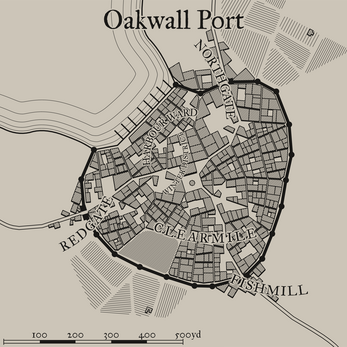
\includegraphics[height = 3 cm]{images/24FsvM.png}\\
     \captionof{figure}\small{Exemple de représentation d'une ville ancienne \\
    provenant de Medieval Fantasy City.}
\end{center}
}
{}
{
\begin{itemize}

\item \textbf{\tab Description : } Vérification que le fichier de sortie correspond à une nouvelle ville ayant pris en compte une génération d'une ancienne ville.\newline
\textbf{\tab Déroulement du test : } On lance le programme et on voit si on génère correctement une ville en ayant garder les anciens bâtiments déjà présents. \newline
\textbf{\tab Entrée : } Un programme de génération de ville aléatoire sur un plan déjà existant. \newline
\textbf{\tab Analyse du test : } Fonctionnement de la génération.

\item \textbf{\tab Description : }Vérification que le fichier de sortie respecte de nouveau les caractéristiques environnementales. \newline
\textbf{\tab Déroulement du test : } On essaie de mettre en place un bâtiment sur une zone qui n'est pas adaptée et on voit si ça fonctionne ou pas.\newline
\textbf{\tab Entrée : } Un programme de génération de ville.

\end{itemize}
}
\besoin{}
{\textcolor{cyan}{Fonctionnalités de l'interface}}
{
L'interface doit pouvoir donner à l'utilisateur l'éventualité de visualiser les éléments de la ville.
\\Dès le lancement il y aura un champs associé à chaque élément de la ville permettant de choisir les spécificités de la ville souhaitée,
en commençant par le nombre de routes principales,  le nombre de structures clés, le nombre de bâtiments et leurs types,
le nombre de montagnes, rivières, lacs et de collines, une fois ces éléments pris en compte, une ville se générera aléatoirement respectant les informations d'entrée.

\begin{itemize}
    \item Posséder un curseur temporel pour observer l'évolution de la ville au cours du temps, c'est à dire que la ville doit s'adapter en fonction de la période choisie par l'utilisateur.
    \item Avoir la possibilité de regénérer une nouvelle ville en écrasant l'ancienne
    \item Avoir la possibilité de choisir les paramètres des éléments, avant la génération de la ville.
    \item Un récapitulatif des données d'entrée.

\end{itemize}
}
{}
{
\begin{itemize}

  \item \textbf{Description : } Vérification que le fichier de sortie correspond à une interface manipulable par l'utilisateur.\newline
  \textbf{Déroulement du test : } On lance le programme et on voit si on génère correctement une interface. \newline
  \textbf{Entrée : } Un programme générant une interface pour l'utilisateur. \newline
  \textbf{ Analyse du test : } Fonctionnement de l'interface.
  
  \item \textbf{ Description : }Vérification que l'interface possède des boutons fonctionnels et impacte la génération de la ville. \newline
  \textbf{Déroulement du test : } On teste le fonctionnement des boutons utilisables sur l'interface. \newline
  \textbf{ Entrée : } Un programme générant une interface pour l'utilisateur.

  \item \textbf{ Description : }Vérification que l'interface prends bien en compte les données d'entrée \newline
  \textbf{Déroulement du test : } On génère des villes avec plusieurs données d'entrée. \newline
  \textbf{ Entrée : } Un jeu de données qu'on rentre dans les différents champs de l'interface. \newline
  \textbf{ Analyse du test : } On vérifie si l'affichage est correct, si les villes dont les données sont les mêmes ont des résultats similaires.
\end{itemize}
}

\newpage

\section{Algorithmes}

\subsection{Routes primaires}
La génération de routes primaire s’effectue grâce à un algorithme de qui génère un nombre de points d’intersection précisé par l’utilisateur aléatoirement 
vers le milieu de la murail, on creer une connexion entre ses points d’intersection d’une façon d’avoir un polygone convexe, on relie alors ses points 
aux portes les plus proche, un point est connecter au plus à deux portes.

\begin{center}
  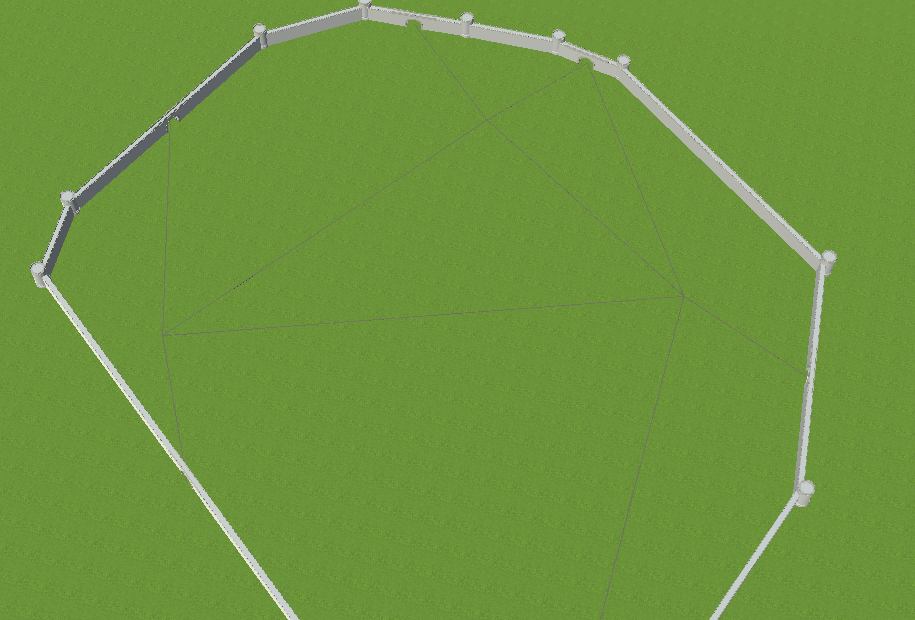
\includegraphics[width = 400px]{images/routeprimaire.png}
  \captionof{figure}{\small{Exemple d'une generation d'une route primaire}}
\end{center}


\subsection{L-systeme pour generation de route}
On va utiliser le système de lindenmayer (L-système) pour faire la génération de routes (principale et secondaire) qui est un système de réécriture qui comprend :

\begin{enumerate}
  \item Un alphabet V : l'ensemble des variables du L-système. On note V* l'ensemble des « mots » que l'on peut construire avec les symboles de V, et V+ l’ensemble des mots contenant au moins un symbole.
  \item Un ensemble de valeurs constantes S.
  \item Un axiome de départ w.
  \item Un ensemble de règles réécriture note P.
\end{enumerate}

Il est possible de construire une suite de mots à partir de l’axiome et des règles de dérivation en remplacant l'axiome par les règles un nombre 
definie de fois. \\

On s’inspire de l’interprétation en tortue \cite{flake2000computational} avec :

\begin{itemize}
  \item F : la tortue avance vers l’avant d’une distance fixe en dessinant un trait.
  \item G : la tortue avance vers l’avant d’une distance fixe sans dessiner de trait.
  \item + : la tortue tourne à droite d'un angle fixe.
  \item - : la tortue tourne à gauche d'un angle fixe.
  \item {[} : enregistrer la position courante de la tortue.
  \item {]} : revenir à la dernière position enregistrée et la supprimer de la pile de positions.
  \item | : la tortue avance vers l’avant d’une distance multipliée par une valeur en dessinant un trait.
\end{itemize}

On se base sur la même interprétation mais on modifie légèrement l’alphabet et on choisit des règles et un axiome propre a notre generation de terrain.
On choisit des valeurs de mouvement aléatoire pour ne pas avoir un même schéma qui se répète.

\textbf{Alphabet :}

\begin{itemize}
  \item F : Créer une route vers l’avant de l’axe Y d’une distance fixe.
  \item + : Créer une route vers la droite d’un angle fixe de 90.
  \item - : Créer une route vers la gauche d’un angle fixe de 90.
  \item {[} : enregistrer la position courante de la route.
  \item {]} : revenir à la dernière position enregistrée et la supprimer de la pile de positions.
  \item | : on avance vers l’avant d’une distance multipliée par une valeur en dessinant un trait.
\end{itemize}

On utilise l’axiome suivant : “+A-B” et pour avoir des routes différente à chaque exécution on utilise plusieur règles :

\begin{center}
  'A',"F[--AE]F[+AE]F" , 'A',"F[++EA]F[-AE]F" , 'A',"F[--EA]F[+AE]F",
\end{center} 

Sur chaque itération on choisit une règle aléatoirement qui nous permet d’avoir les résultats ci dessous.

\begin{center}
  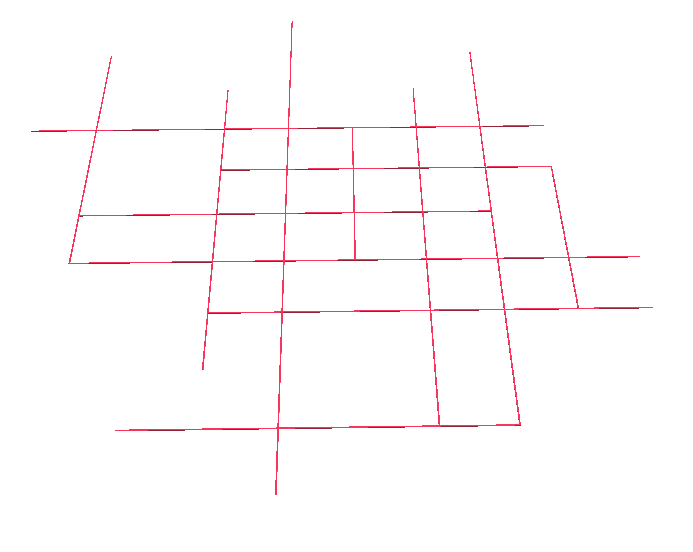
\includegraphics[width = 200px]{images/lsystem1.png}
  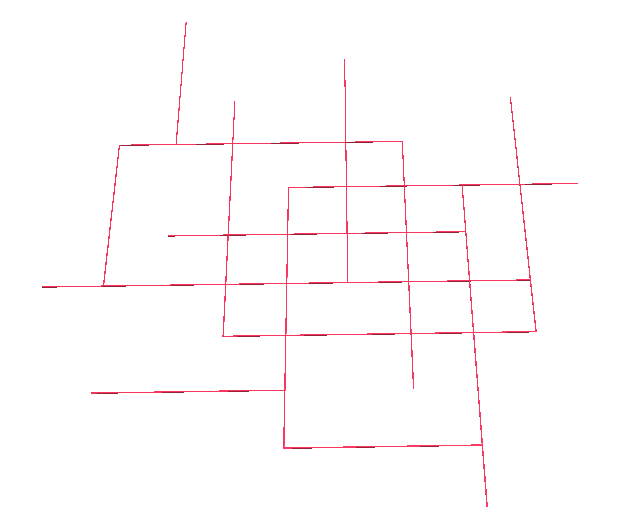
\includegraphics[width = 200px]{images/lsystem2.png}
  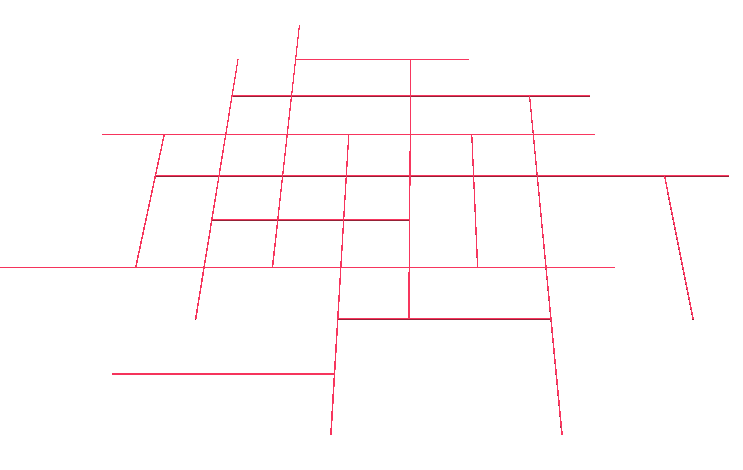
\includegraphics[width = 200px]{images/lsystem3.png}
  \captionof{figure}{\small{Exemple plusieur execution L-systeme}}
\end{center}

\newpage

\subsection{création de muraille qui entoure la ville}

L’algorithme nous permet principalement de définir l’endroit de la ville sur la map déjà générée qui se déroule comme ceci :\\

On commence par générer un point aléatoire vers le centre de la carte en divisant x et y par 2, on prend une valeur aléatoire qui servira de rayon aléatoire pour créer un cercle du point qu'on a pris comme centre. \\

On fait des pas aléatoire sur le périmètre du cercle qu'on vient de créer, c’est à dire qu’on se met aléatoirement sur une position du périmètre et on change l’angle, on aura des coordonnées $x$ et $y$ comme ceci $X =  rayon * cos(angle)$ | $Y = rayon * sin(angle)$.

Le fait de changer l’angle aléatoirement nous fait avoir des points $X$ $Y$ sur le long du périmètre du cercle, pour faire une plus grande variation entre les jonctions de la muraille, on crée depuis ses points des cercles avec un rayon plus petit que le rayon du premier grand cercle.

Pour chaque petit cercle créé sur le périmètre du premier grand cercle on génère un point aléatoire qui est défini par un angle et un rayon plus petit que le rayon du cercle.

\begin{center}
  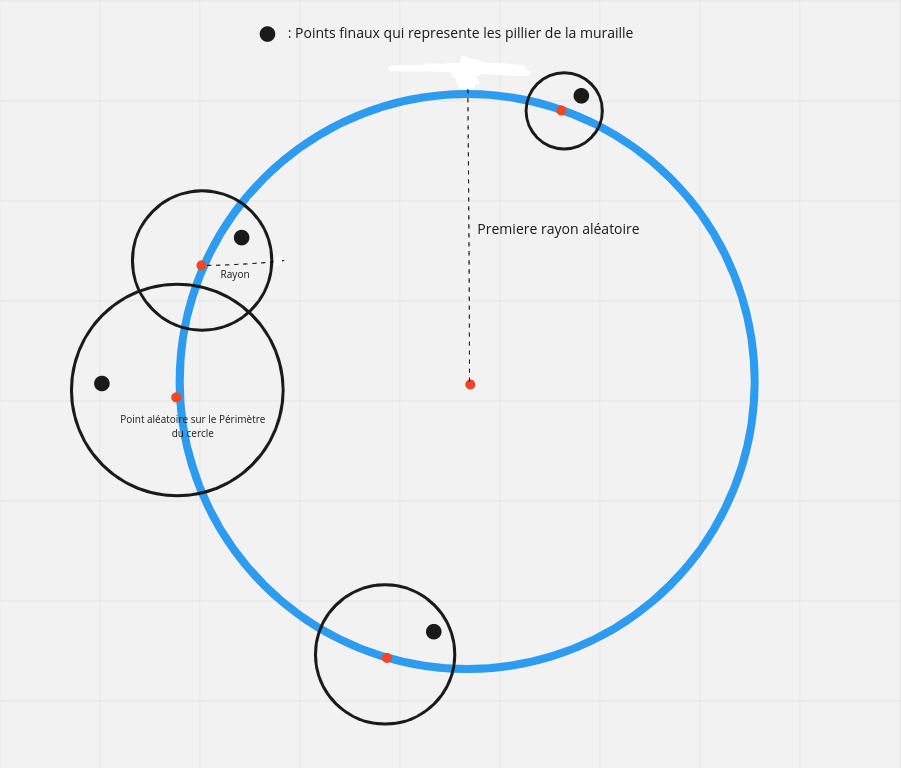
\includegraphics[height = 6 cm]{images/algorithme.png}
  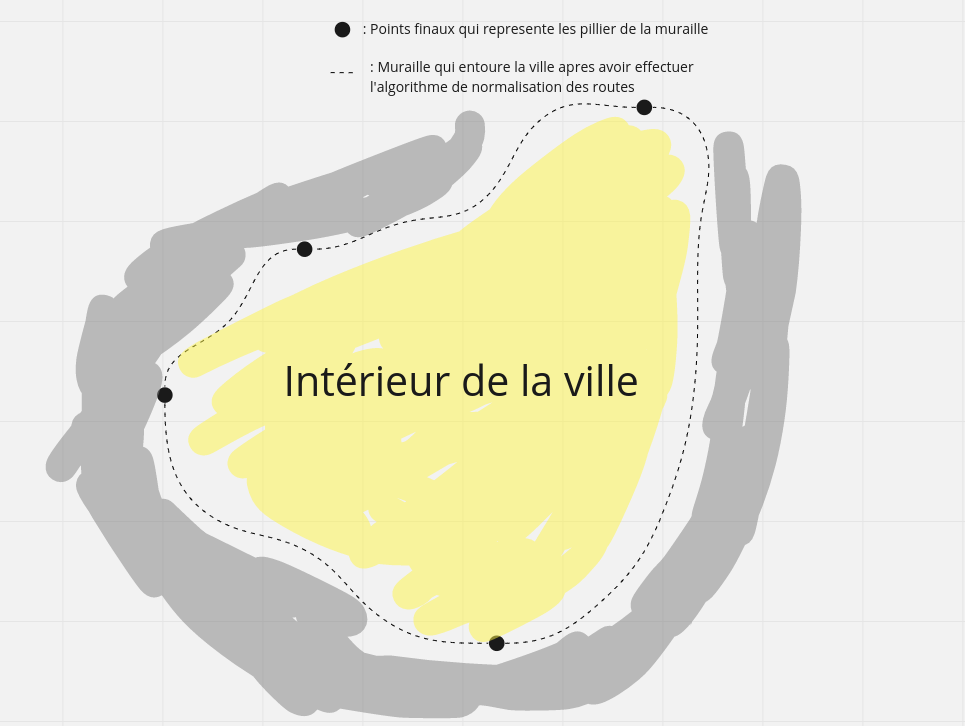
\includegraphics[height = 6 cm]{images/algo_final.png}\\
  \captionof{figure}{\small{ Déroulement de l'algorithme}}
\end{center}

\subsection{Algorithme d'échantillonnage}

Pour chaque point représentant le début A et la fin B d’une route, on prendra un rectangle d’une longueur à définir et d’une largeur de la taille entre A et B. On peut tracer le rectangle grâce au vecteur (A,B) qui nous permettra d’avoir le milieu.
On utilisera une de ses stratégies de sélection d'échantillonnage de routes pour sélectionner le chemin à prendre :\\

\begin{itemize}
  \item Stratégie d'élévation minimale : sélection de l'échantillon avec l'élévation (axe Z) la plus faible.
  \item Différence d'élévation la plus faible : On évite les chutes ou les montées d'altitude, et on cherche à maintenir une altitude régulière pour le segment de route complet. 
  \item Différence d'élévation moyenne : on sélectionne les points qui font une moyenne d’altitude.
\end{itemize}

Les trois stratégies sont contraintes d’avancer vers le point final en testant pour chaque nouveau point si on approche du point final.
Le choix se fait du prochain point se fait aléatoirement tant qu’il maintient une distance d’un seul point avec le points déjà selectionner.

Après la generation des points de murail on prends aléatoirement un nombre de porte qu’on crée au milieu des murs choisis aussi aléatoirement.

\begin{center}
  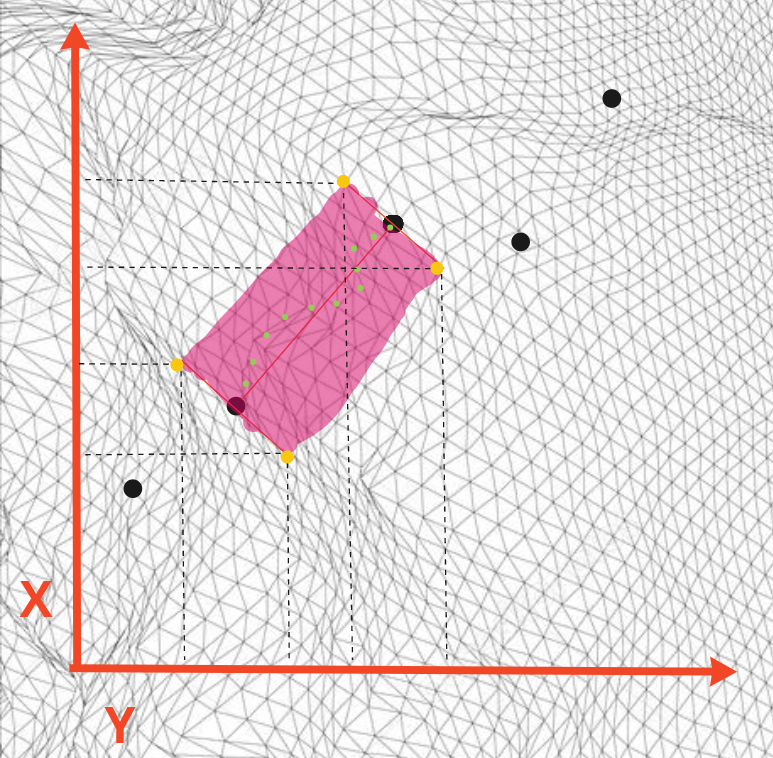
\includegraphics[height = 8 cm]{images/algo.png}\\
  \captionof{figure}{\small{ Déroulement de l'algorithme}}
\end{center}

\subsection{Algorithme de génération de bâtiments}

La génération de bâtiment se fait grâce à une bibliothèque de modèles médiévaux \cite{Assets}, elle contient plusieurs modèles qu’on va utiliser comme des bâtiments, arbres, etc.

La génération de bâtiments se fait en premier lieu autour des routes primaires et secondaires, grâce aux deux points qui représentent 
le début et la fin de la route, on peut obtenir la direction et la longueur qui nous permet de placer les bâtiments sur les deux côtés de la route, 
l’orientation se fait grâce au produit croisé du vecteur z avec la direction .
Les bâtiments sont placés d'un espace fixe de la route et d'un espace aléatoire des autres bâtiment précisé par l'utilisateur.

\begin{algorithm}
  \caption{Generer batiment}
  \KwData{Vecteur pointA, Vecteur pointB}
  
  float distance = pointB - pointA\;
  Vecteur orientation = cross((pointA - pointB) , (0,0,1))\;

  \For{int i = 0 ; i < distance ; i += tailleBatiment}
  {
    int position = Random(-espace,espace)\;
    i += position\;
    AfficherBatiment(pointA, position, orientation)\;
  }

  return;
\end{algorithm}

\newpage

\subsection{Algorithme de création de relief}

L’algorithme de l’interpollation linéaire (à ne pas confondre avec l’interpolation cubique qui lui lisse le relief) consiste à ajouter une courbe dans laquelle on a établi des points de pic ou de creux , pour établir une surface en relief, dans laquelle on y ajoutera des textures pour ressembler le plus à la description de l’objet que l’on veut établir , on va parler de bruits de turbulences, qui vont permettre d’ajouter le plus de détails possible à l’objet. Pour établir ce bruit on utilisera l’algorithme Perlin Noise : le but de cet algorithme et de créer une texture que l’on pourra utiliser comme effet visuel pour augmenter le réalisme de l’objet utilisé. L'algorithme peut être utilisé avec plusieurs dimensions et il consiste à calculer la produit scalaire de vecteurs gradiants que l'on aura mis en place sur une grille au préalable et de créer une interpolation de ces valeurs pour obtenir de nouvelles coordonnées et ainsi avoir un relief.

On va créer à partir d'un nuage de point de coordonnées (x,y) une fonction établissant la courbe entre chacun de ses points : 

La fonction $\bar{f}$ est définie par

\begin{center}
  ${\displaystyle {\bar {f}}(x)={\frac {y_{a}-y_{b}}{x_{a}-x_{b}}}x+{\frac {x_{a}\cdot y_{b}-x_{b}\cdot y_{a}}{x_{a}-x_{b}}}}$ \\
\end{center}

Une fois les calculs établis on obtient une courbe qui va alors nous permettre de créer un terrain en relief : 

\begin{center}
  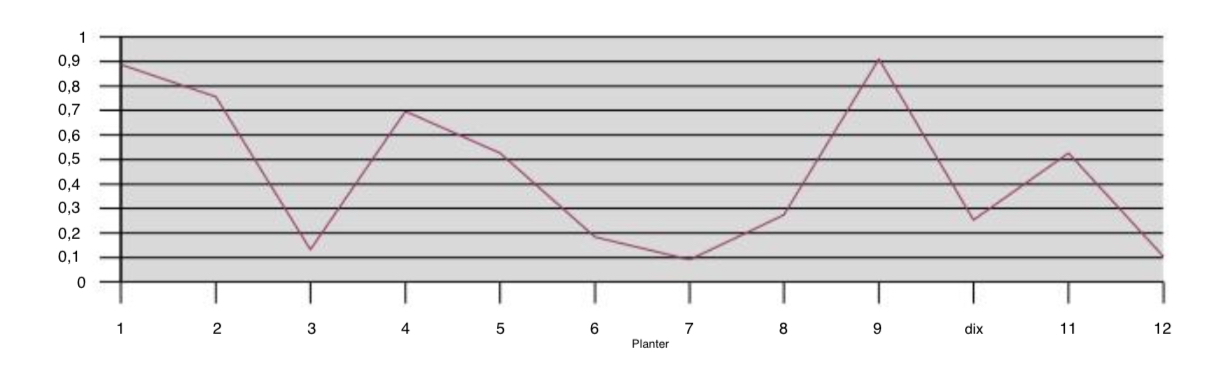
\includegraphics[height = 4 cm]{images/interlineaire.jpeg}\\
  \captionof{figure}{\small{Exemple de courbe par l'interpolation linéaire}}\cite{Kelly}
\end{center}

Le principe de l'interpolation s'établi à partir d'une formule qui peut être quelconque, le but est simplement d'obtenir de nouvelles valeurs de x et y, la formule ne doit pas être linéaire car on cherche à obtenir un terrain en relief et donc des coordonnées de hauteurs différentes pour chaque point, elle doit aussi donner des résultats similaires pour éviter d'avoir de trop grands écarts entre chaque point et ainsi obtenir un relief qui a des points trop elevés et d'autre trop faibles.

\subsection{Bruit de Perlin pour la création de relief}
On va utiliser le bruit de Perlin pour créer la génération du terrain.  

Le bruit de Perlin est une formule qui permet de créer une texture procédurale utilisée pour créer un effet visuel de réalisme. La fonction a une apparence de pseudo-aléatoire, mais c'est tout à fait le contraire, la texture produit un rendu "désordonné".

L'algorithme consiste à former une fonction de bruit qui, à une valeur donnée, associe une valeur qui semble aléatoire. Les valeurs obtenues sont donc liées aux valeurs de rentrée. 

Le résultat pourra être reproduit dans une deuxième texture si on insère les mêmes valeurs utilisées pour générer la texture précédente (à moins que le changement soit voulu ou effectué par un algorithme tierce).\\

C'est l'utilisation des paramètres tiers qui nous permettra d'obtenir un jeu de valeurs aléatoires pour qu'un observateur ne puisse pas trouver un motif qui se répète à certains intervalles. La difficulté réside dans le fait qu'on doit créer des valeurs aléatoires qui ont un rendu "désordonné". 

L'algorithme se décompose en deux étapes:
\begin{enumerate}
	\item Grille avec les gradients aléatoires : 
		l'algorithme forme une fonction f:N -> R qui, à une valeur donnée associe une valeur qui semble aléatoire. Cette caractéristique permet de reproduire le même résultat dans une deuxième texture si on insère les mêmes valeurs utilisées pour générer la texture précédente (à moins que le changement soit voulu ou effectué par un algorithme tierce).\\

\begin{center}
    \centering
    
\includegraphics[height = 3 cm]{images/Perlin_noise.jpg}
    \captionof{figure}{Bruit de Perlin en deux dimensions \cite{berlinNoise}}
\end{center}

	\item Interpolation : 
	L'interpolation est « une opération mathématiques permettant de construire une courbe à partir des données d'un nombre fini de points ». Cette opération nous permet de créer une structure connectant chacune des coordonnées entre elles et produire un "maillage" qui sera utilisable lors de la création d'une surface.

\end{enumerate}

\begin{center}
    \centering
    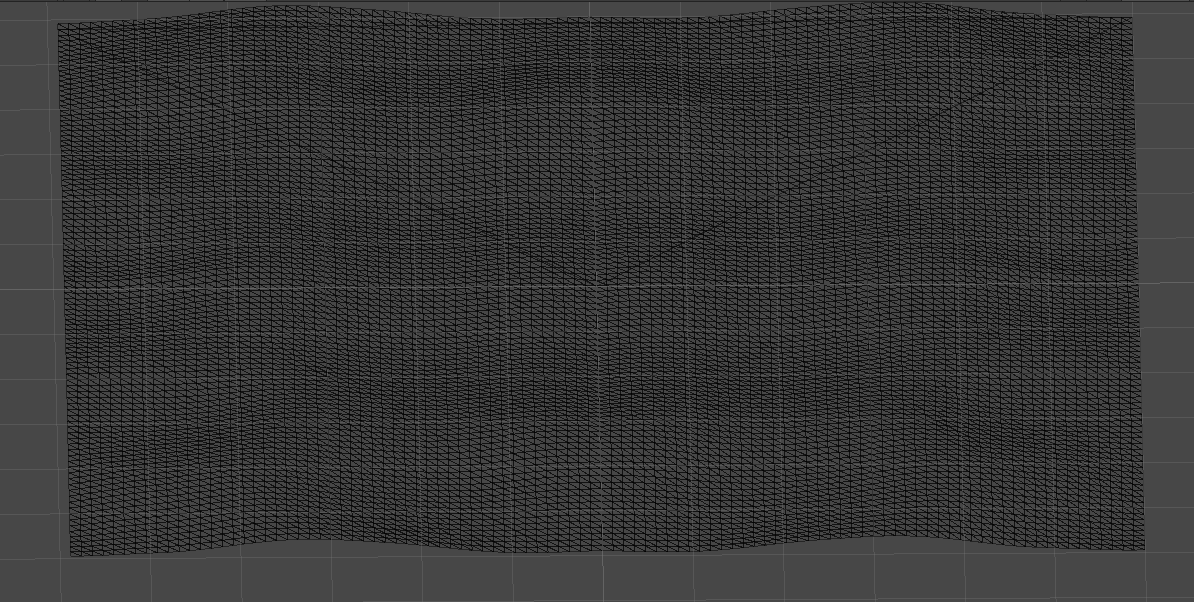
\includegraphics[height = 3 cm]{images/exemple_maillage.png}
\end{center}


Pour rendre le résultat avec plus de détails on peut implémenter les modifications suivantes: 

\begin{itemize}

\item Amplitude: Si on regarde la courbe point d'un point A à un B du terrain on observe que les valeurs (x, y, z) forment une courbe, le problème de ce dernier c'est que le terrain manque de perturbations.
	
     Pour cela on utilisera des octaves pour créer une irrégularité dans la texture. Les octaves c'est l'ensemble de courbes (créées par le bruit de Perlin) qui vont être utilisées pour former une courbe de forme quelconque. Pour cela on utilisera de la lacunarité et la persistance.
    
\item Lacunarité: Chaque octave pose une fréquence différente, donc les courbes produites sont différentes les unes des autres. La courbe utilisée pour créer une montagne doit avoir une fréquence plus grande que celle d'une colline car si la fréquence d'une montagne est petite avec une altitude élevée alors on obtient un pic dans le terrain.

\begin{center}
\centering
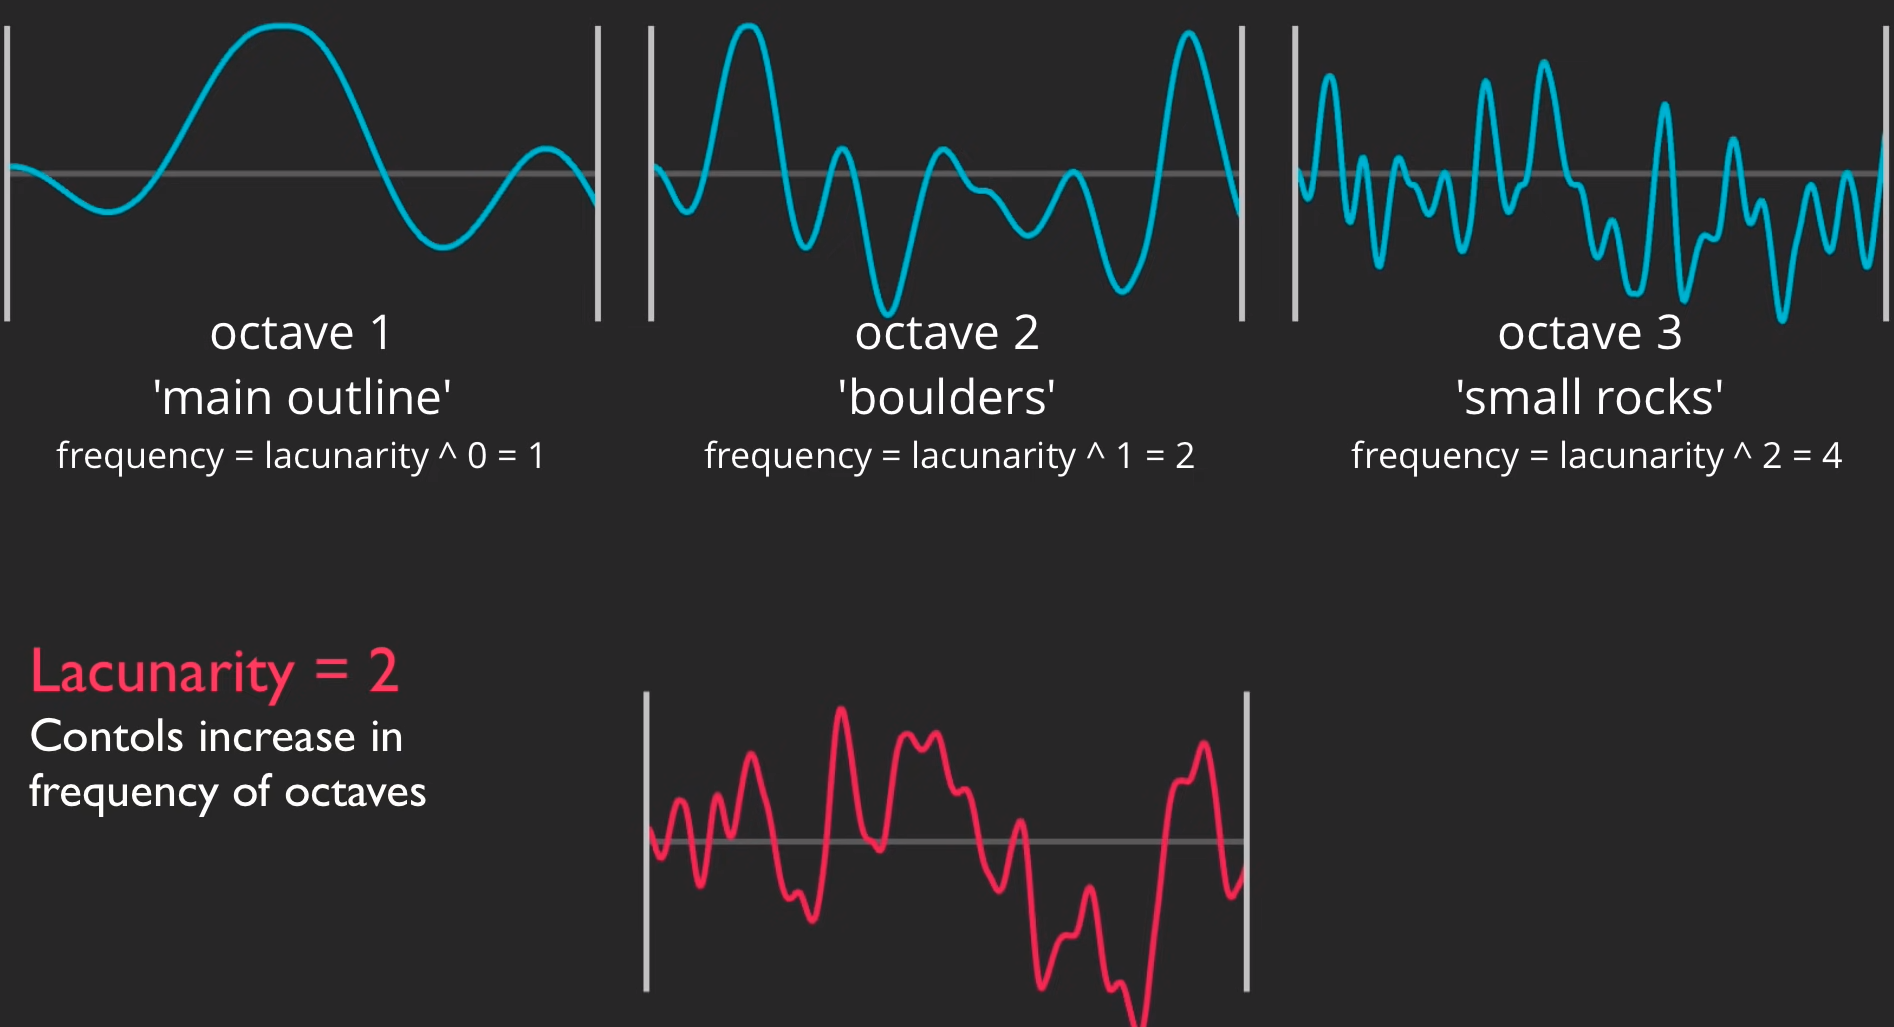
\includegraphics[height = 3 cm]{images/lacunarity.png}
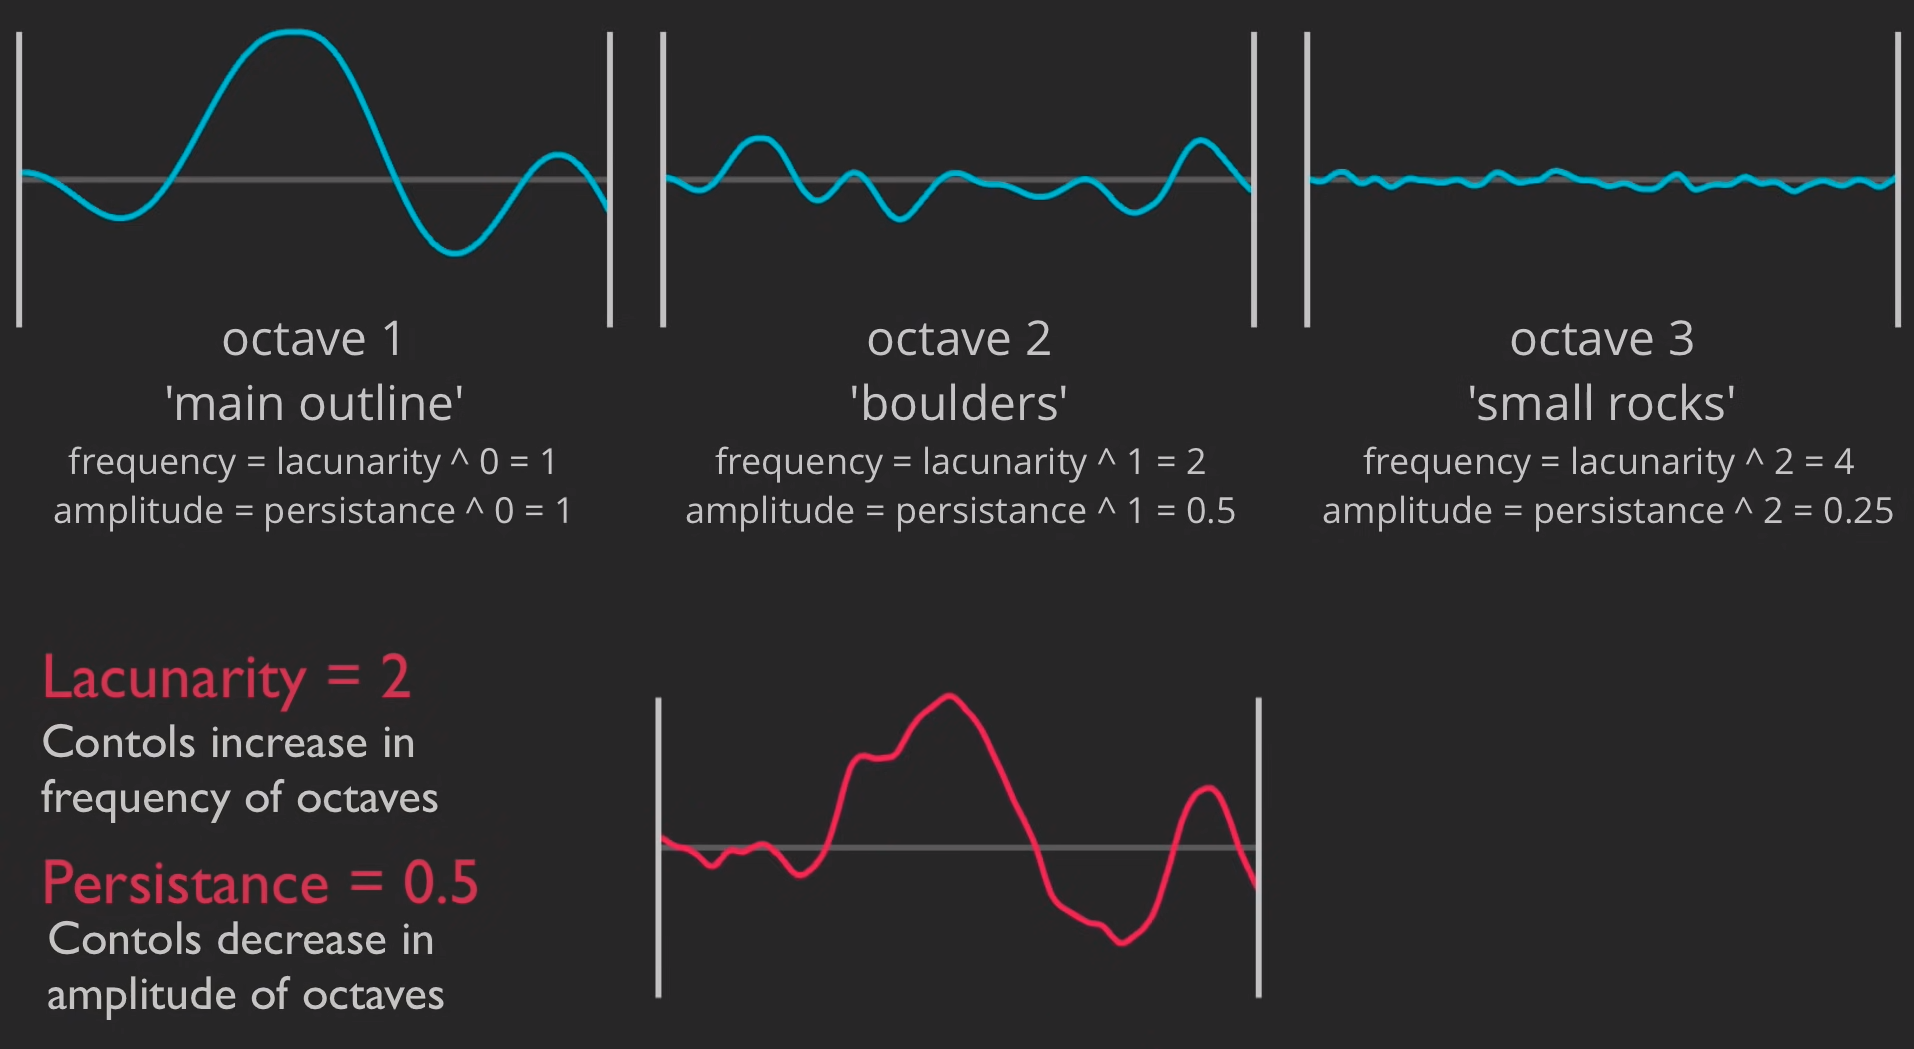
\includegraphics[height = 3 cm]{images/persistance.png}\\
\captionof{figure}{\small{Courbe bruit de Perlin avec amplitude.} \cite{lewisUnity}}
\captionof{figure}{\small{Courbe bruit de Perlin avec persistance.} \cite{lewisUnity}}
\end{center}

\item Persistance: c'est la fréquence (ou influence) des octaves sur la courbe principale. Chaque octave possède une importance sur le terrain, c'est-à-dire, l'octave qui sera utilisée pour 
créer des imperfections superficielles était moins importantes que l'octave utilisée pour ajouter des collines. 

\end{itemize}

\begin{center}
    \centering
    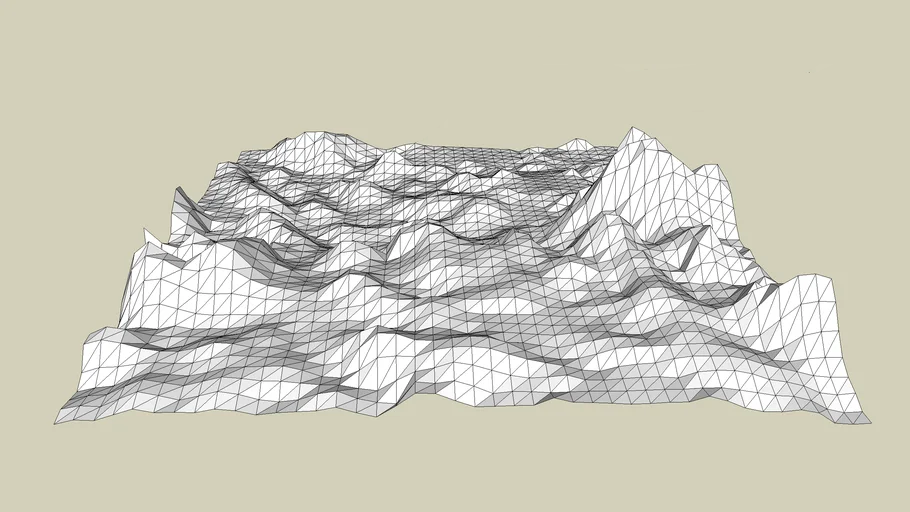
\includegraphics[height = 3 cm]{images/terrain3d.png}\\
    \captionof{figure}{\small{Exemple de représentation d'un terrain.} \cite{modelTerrain}}
\end{center}

Après avoir suivi les étapes précédentes on devrait avoir un terrain utilisable pour commencer à contruire les routes et le village.


La génération du terrain est un système qui comprend : 

\begin{itemize}
  \item Un tableau de taille (longueur x largeur) avec la valeur de la hauteur du point dans le terrain.
\end{itemize}

La tableau sera généré grâce à la fonction Mathf.Noise (fonction dans les bibliothèques de l'application Unity (moteur de jeu)) qui nous permet d'obtenir une suite de valeurs en utilisant la fonction du Bruit de Perlin.

\begin{center}
  
\includegraphics[width = 200px]{images/bruit_perlin_unity.png}
  \captionof{figure}{\small{Exemple d'une image produite sur unity en utilisant le bruit de Perlin}}
\end{center}

L'image est analysée de la manière suivante : la hauteur est codée avec une valeur allant de 0 à 1, plus on se rapproche de 0 plus on aura une couleur blanche et plus on se rapproche du 1 plus on aura une couleur noire.

\begin{algorithm}
  \caption{Bruit de Perlin}
  \KwData{coordonnées x, y}
  \KwResult{coordonnées x, y}
 
  initialisation \;
  
  grille[k] = (x,y); //vecteur gradiant
  
  \For{int i = 0; i < n; i++}{
  	distance[i] = |grille[i] - grille[k]| //vecteur distance \;
	int x1, y1 = produitScalaire(grille[k],distance[i]) \;
	interpolation(x1, y1)
  }
  	retourner x1\, y1\;
\end{algorithm}
% Algo MCB

\subsection{Algorithme MCB}
  
  L’algorithme MCB (Monte-Carlo Localization Boxed) nous permet de créer les City Cells en déterminant les boucles fermées du graphe des routes primaires.\\
  La création d'une liste d’adjacence de tout chaque points des routes principales nous permet d’avoir toutes les connexions des points.
  On commence par un point A et le un point B de sa liste d’adjacence, on prend la list d’adjacence du point B et on prend le point après 
  le point A, si le point A est a la fin de la list on prend le premier point de la list, jusqu'à retrouver le point A.

  Cet Algorithme nous retourne une liste de point qui forme les cellules de la ville, ce qui vas etre utile pour afficher les routes secondaire dedans.
   
  \begin{algorithm}
    \caption{Algorithme MCB}
    \KwData{List<Vecteur> listAdjacence , Vecteur pointA, Vecteur pointB}
    \KwResult{List<Vecteur> cellule}
    Vecteur pointDepart = pointA\;
    bool trouver = false\;

    \While{!trouver}
    {
      cellule.Ajouter(pointA);

      \ForEach{point dans listAdjacence[pointB]}
      {
        \If{!premiereExecution() and listAdjacence[pointB].contient(pointDepart)}
        {
          trouver = true;
        }
        \If{point == pointA}
        {
          Vecteur prochainPoint = point.Prochain();
          pointA = pointB;
          pointB = prochainPoint;
        }
      }
    }

    return listAdjacence\;

  \end{algorithm}
  
  
\begin{center}
  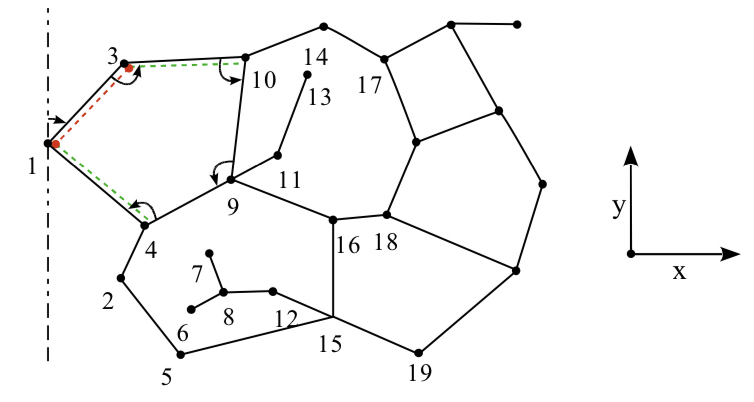
\includegraphics[height = 7 cm]{images/MCB.png}\\
  \captionof{figure}{\small{L'algorithme MCB \cite{Kelly}}}
  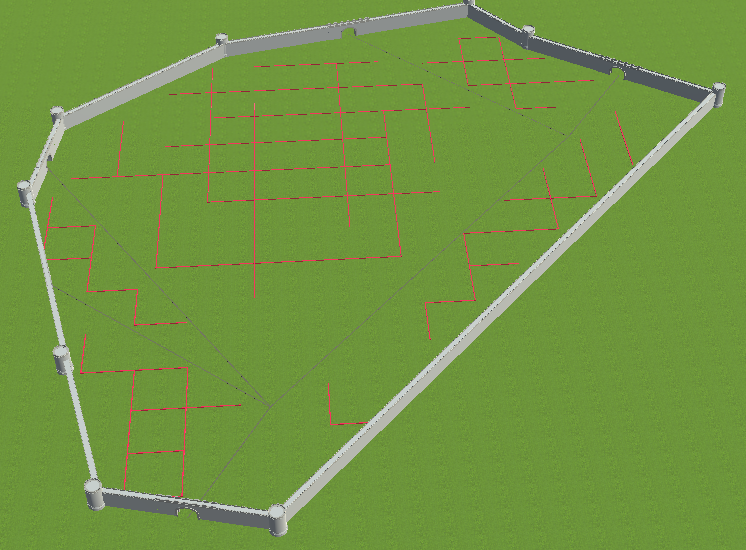
\includegraphics[height = 7 cm]{images/routeprimaireetsecondaire.png}\\
  \captionof{figure}{\small{Utilisation de cellules pour generer routes secondaire}}
\end{center}



\newpage

\section{Architecture}

L'architecture du code de notre projet se présente sous forme de diagramme dans lequelle on retrouve dans un premier temps deux sections sginificatives : une qui concerne les infrastructures avec les constructions humaines tel que les routes, les bâtiments, et la muraille; et une autre qui concerne le terrain et les éléments environnementaux qui le compose comme les arbres, l'herbe etc..

\begin{center}
    \centering
    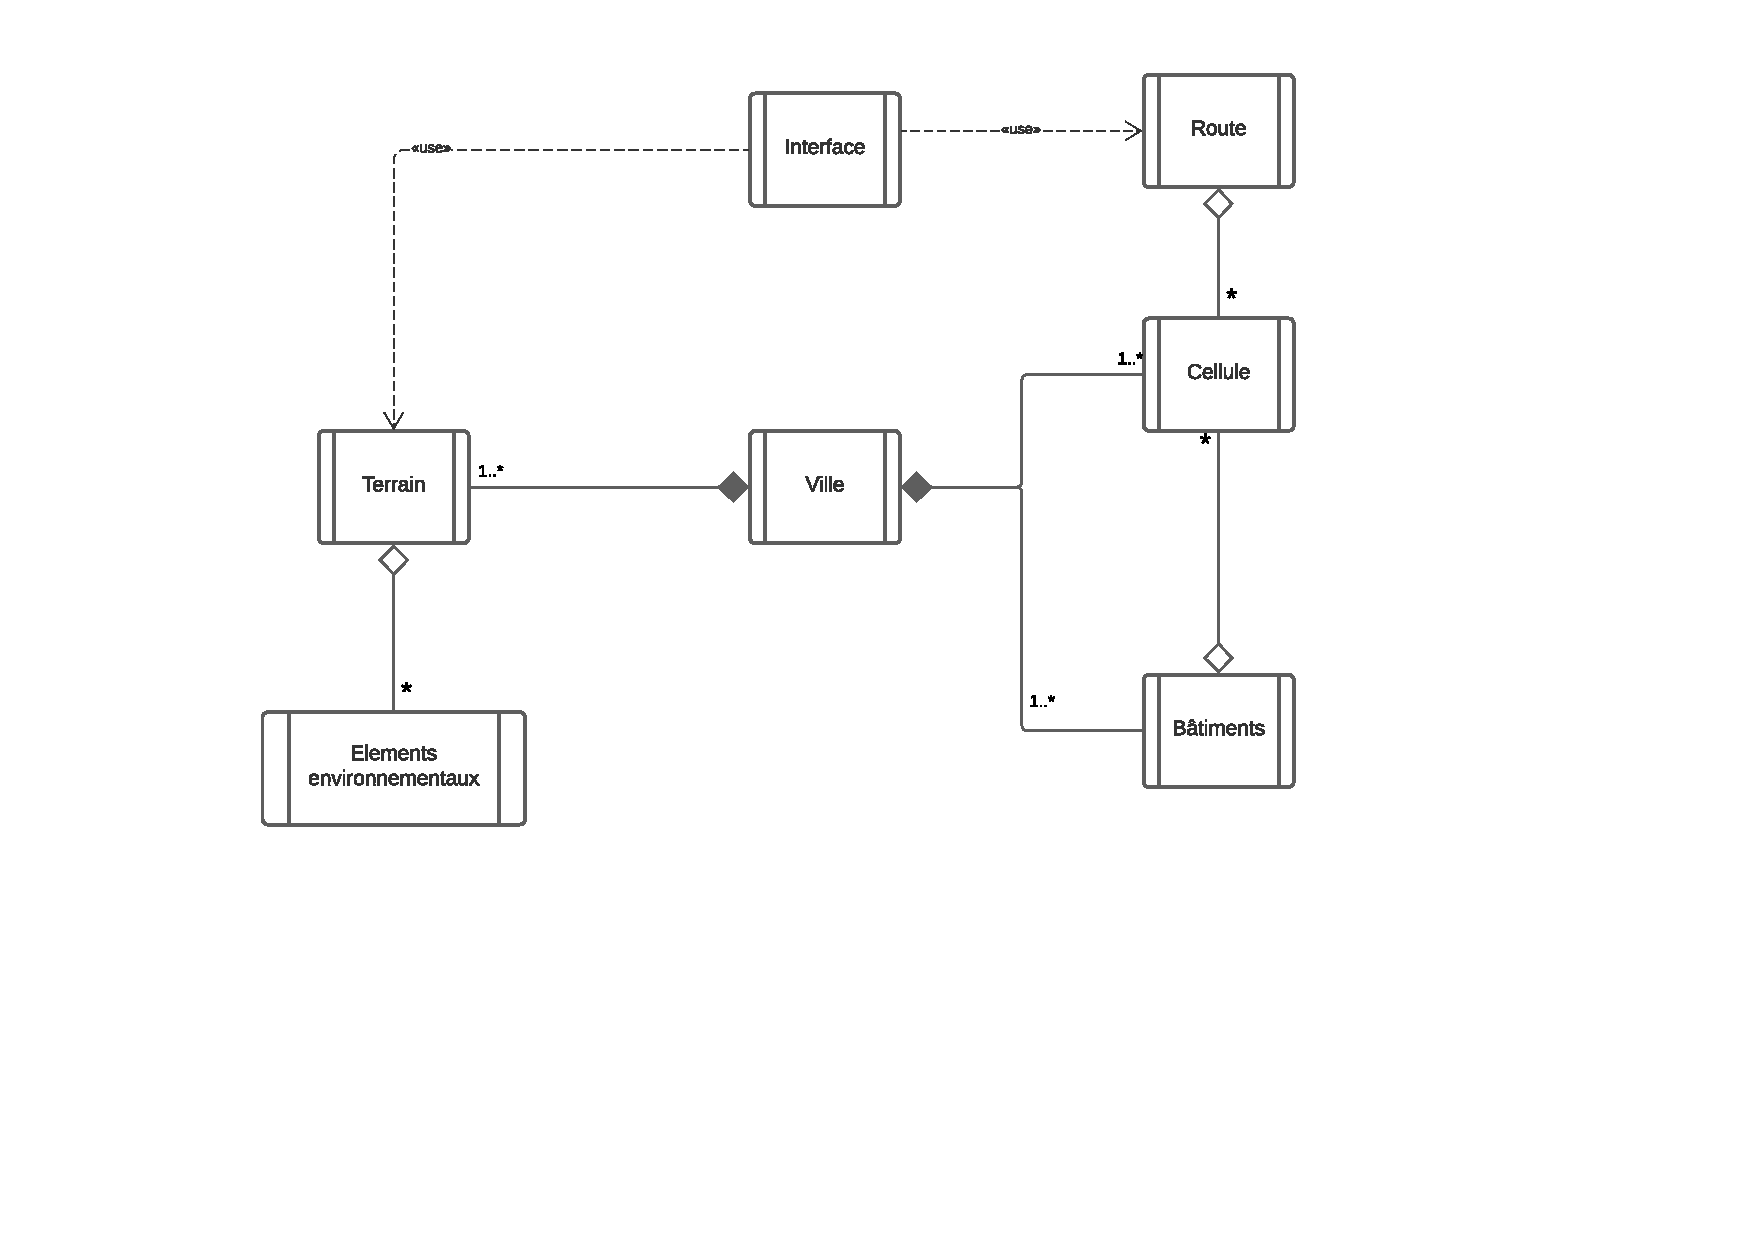
\includegraphics[height = 8 cm]{images/DiagrammeSimple.pdf}\\
\end{center}

Il existe également une autre version de notre architecture qui cette fois-ci est beaucoup plus précise puisqu'elle se compose des classes principales de notre code à savoir :
\begin{itemize}
	\item Générer une ville qui va faire appel à générer un terrain, des bâtiments, des routes et des cellules.
	\item Le terrain qui va générer une surface en relief grâce au bruit de Perlin, des rivières et de la végétation comme des arbres et de l'herbe.
	\item Les bâtiments qui vont être générés par type de bâtiment et sur des cellules dans lesquelles on va également générer les routes.
	\item Une interface utilisateur qui met en place des informations comme générer le nombre de bâtiments, de routes, etc..
\end{itemize}

\begin{center}
    \centering
    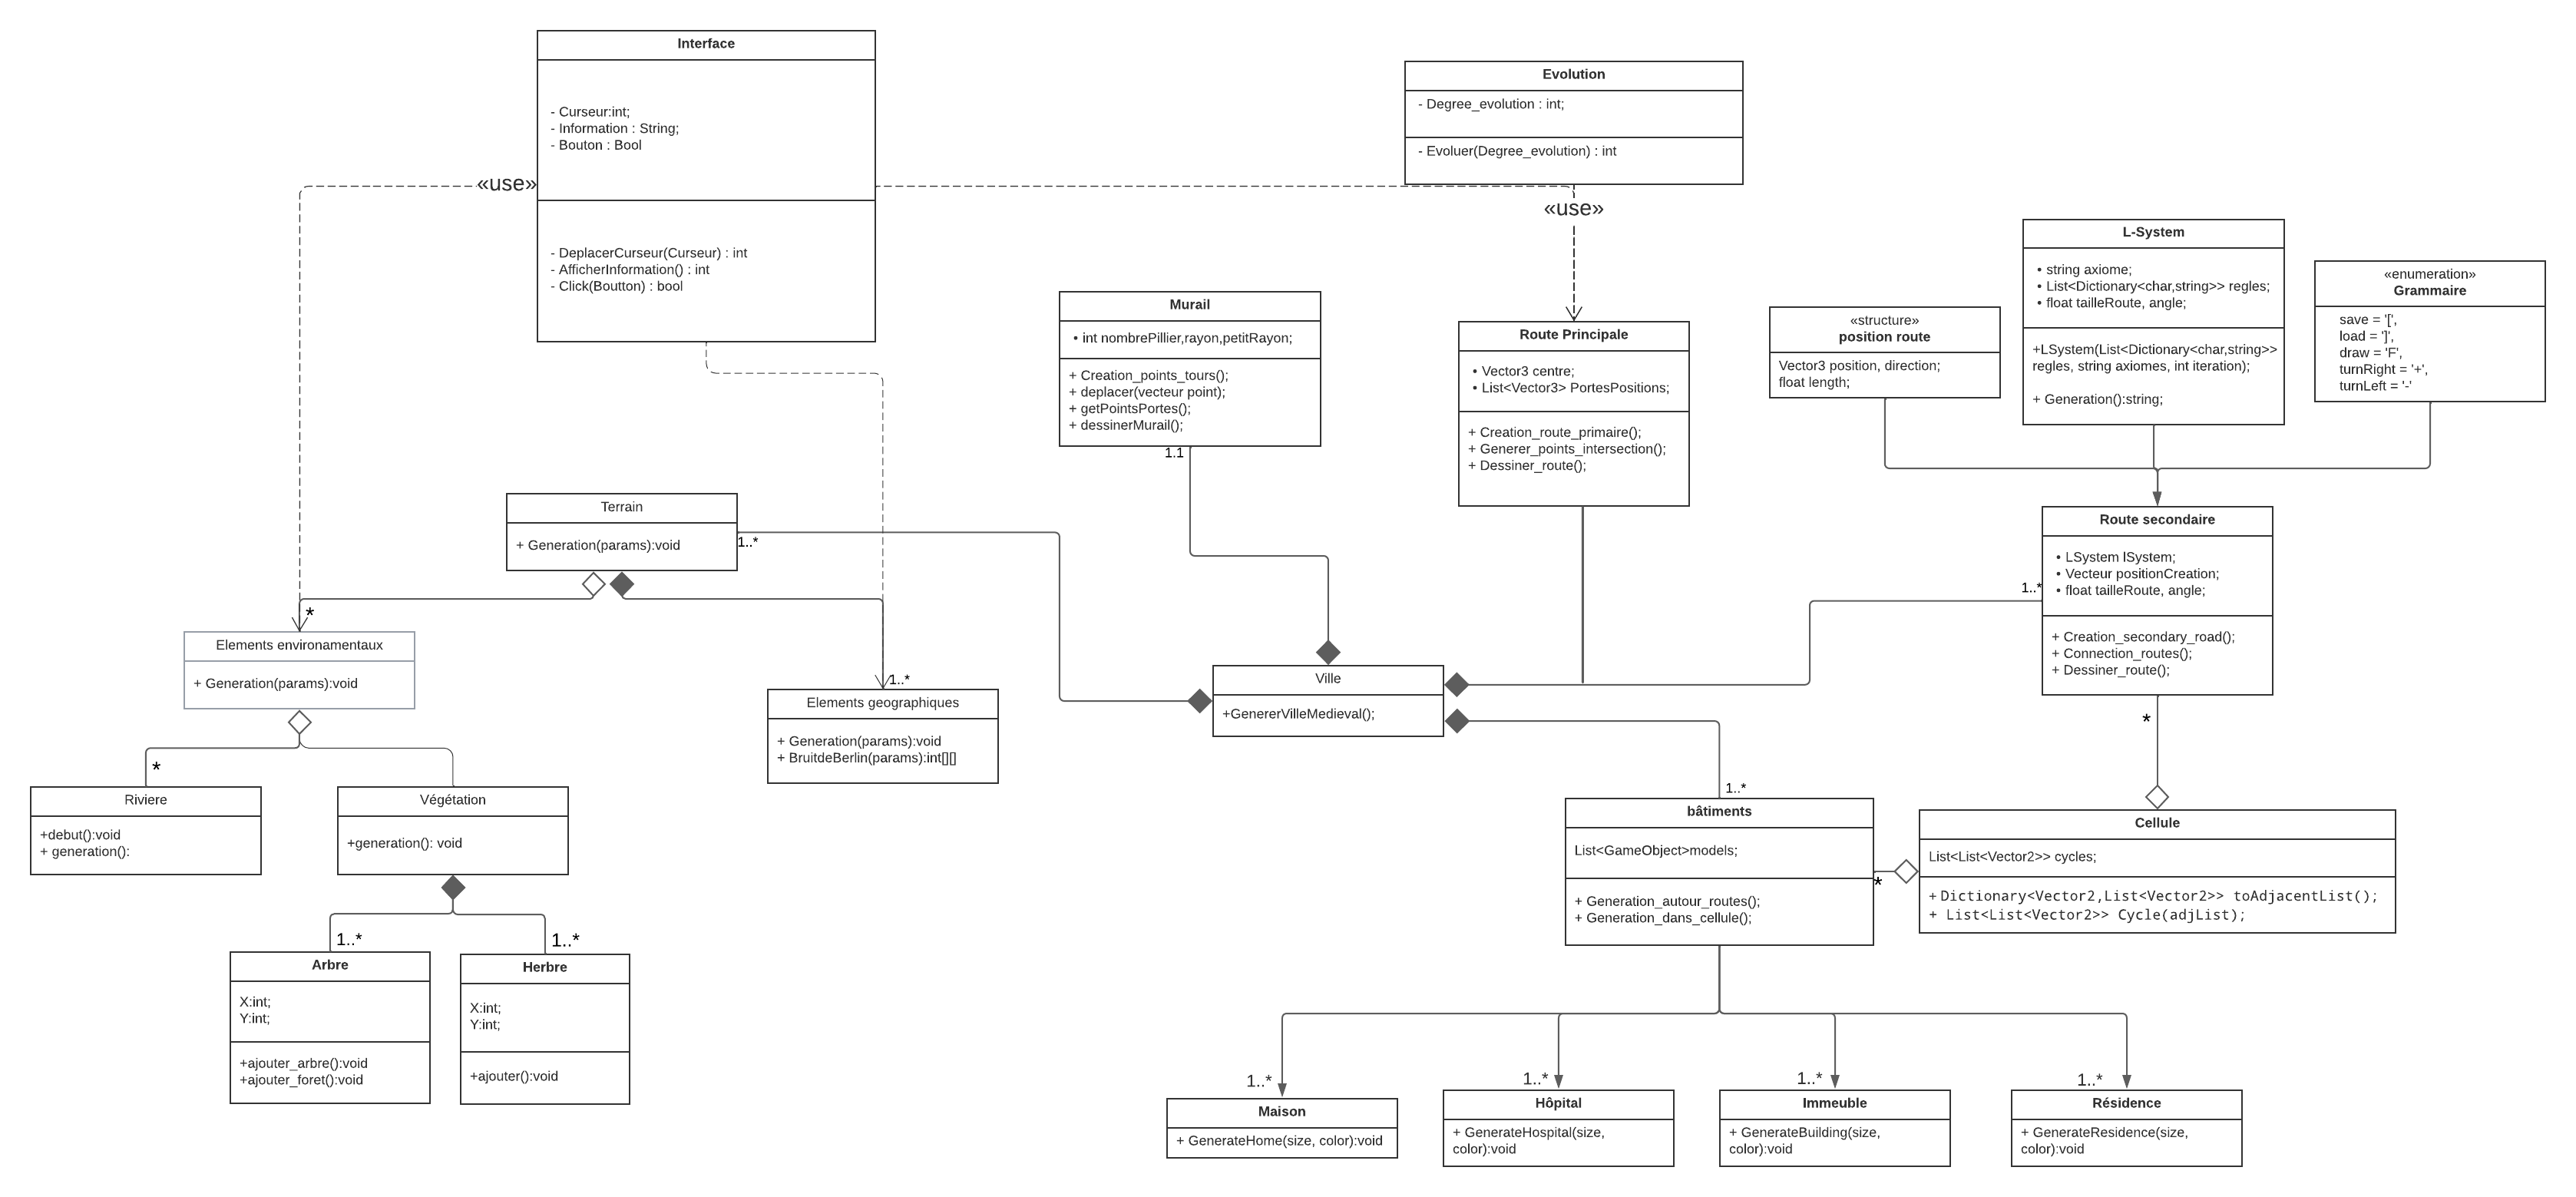
\includegraphics[height = 13 cm, angle = 90]{images/Diagramme_V5.png}\\
\end{center}

\newpage

\section{Le moteur Unity}
\subsection{\textbf{Introduction}}

Unity est un moteur 2D/3D de développement temps réel, aujourd’hui largement répandu dans l’industrie du projet vidéo grâce à ses boîtes à outils particulièrement fournis permettant la création d’expériences interactives 2D, 3D.\\
En plus d'être un moteur de projet 2D/3D, Unity est également un environnement de développement intégré (IDE). Ainsi, il rassemble divers outils de développement que les développeurs utilisent souvent dans une interface graphique.\\
Par conséquent, la plateforme met à disposition un éditeur visuel qui offre la possibilité de simplement faire glisser et déposer différents éléments dans la scène. Qu'on peut ensuite modifier comme on le souhaite.\\
Le choix de ce moteur nous semble donc évident pour satisfaire nos besoins.

\subsection{\textbf{Fonctionnement interne et outils de développement}}

Unity \cite{unity} est un moteur de projet basé sur du C++ mais l'écriture du code est en C sharp, ce dernier permet de tester dans l'IDE sans aucun type d'exportation ou de construction. Lorsqu'on exécute notre code dans Unity, on utilise Mono version 3.5, qui a une compatibilité API à peu près équivalente à .NET Framework 3.5/CLR 2.0.\\
On peut utiliser MonoDevelop pour le débogage ou utiliser des plugins tiers pour Visual Studio, UnityVS.\\
MonoDevelop a un plugin qui ouvre une connexion au débogueur Unity et lui envoie des commandes après le débogage.\\

\subsection{\textbf{Un système de pipeline}}

Un système de pipeline \cite{pipeline} est un système qui permet de contrôler et d'adapter le rendu grâce à des scripts en C Sharp.\\

Sur Unity, il y a le choix entre trois systèmes de pipeline prédéfinis.\\

Le pipeline de rendu intégré standard est le pipeline de rendu par défaut de Unity. Il s'agit d'un pipeline de rendu à usage général qui dispose d'options de personnalisation limitées.\\

Le pipeline de rendu universel (URP) est un pipeline de rendu scriptable qui est rapide et facile à personnaliser et permet de créer des graphiques optimisés sur une large gamme de plateformes.\\

Le pipeline de rendu haute définition (HDRP) est un pipeline de rendu scriptable qui permet de créer des graphiques haute fidélité de pointe sur des plateformes haut de gamme.\\

On peut également créer notre propre pipeline de rendu à l'aide de l'API Scriptable Render Pipeline d'Unity.\\

Chacun des différents systèmes pipeline cible des types d'utilisations et des besoins matériels bien précis.\\

Dans notre cas on utilisera le pipeline de rendu intégré standard.

\subsection{\textbf{L'interaction avec la carte graphique}}

Le matériel graphique \cite{graphic} qui rend finalement la scène est contrôlé par un programme graphique spécial appelé Shaders. Les fonctionnalités matérielles sont progressivement améliorées au fil du temps et les fonctionnalités communes introduites à chaque étape sont appelées modèles de Shader. Le modèle de Shader progressif ajoute la prise en charge de programmes de shader plus longs, d'instructions de branchement plus puissantes et d'autres fonctionnalités, et ces améliorations permettent des améliorations parallèles des graphiques.\\

Unity permet d'obtenir des rendus graphiques en utilisant un modèle Shader inférieur ou au mieux aussi puissante que la carte graphique utilisée. \\

On peut également choisir le niveau d'émulation graphique, ceci est utile pendant le développement pour voir à quoi ressembleront les graphiques sur une machine plus ancienne.\\

Les performances de processeur au GPU (Graphics processing unit) diminuent jusqu’aux appels de dessin soumis à la carte graphique. Pour améliorer les performances, les appels de dessin doivent être stratégiquement réduits ou bien structurés afin d’obtenir des résultats optimaux. Étant donné que les appels de dessin eux-mêmes sont pleins de ressources, leur réduction réduira le travail global nécessaire. 

\subsection{\textbf{Lots d'appels de dessin}}

Le lot d'appels de dessin \cite{dessin} est une méthode d'optimisation des appels de dessin qui combine des maillages afin que Unity puisse les rendre en moins d'appels de dessin possible. \\

Unity fournit deux méthodes intégrées de traitement par lots des appels de dessin :\\

\textbf{- Traitement par lots statique} pour les GameObjects statiques, Unity les combine puis les assemble pour obtenir un rendu.\\

\textbf{- Mise en lot dynamique} pour les maillages suffisamment petits, cela transforme leurs sommets sur le CPU, regroupe les sommets similaires et les restitue en un seul appel de dessin.

\begin{center}
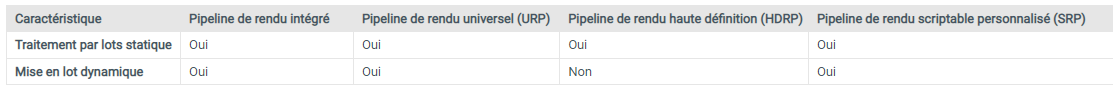
\includegraphics[height = 1.5cm]{images/pipeline.png}\\
\captionof{figure}{\small{Compatibilité du pipeline de rendu issue de la documentation officiel d'Unity}}
\end{center}

\subsection{\textbf{Version de logiciel utilisé}}

Les nouvelles versions \cite{version} disposent de fonctionnalités dont on aura pas besoin, on a donc choisi de travailler sur Unity version 2020.3.32f1 car cette version est stable et dispose de tout ce dont on a besoin afin de mener à bien notre projet.

\newpage

\section{Fonctionnement}

\subsection{Interface}

Notre génération de ville se présente par une interface dans laquelle il est possible d'opter pour deux options :
		- générer une ville aléatoirement 
		- paramétrer la ville que l'on veut générer

\begin{center}
	\centering
    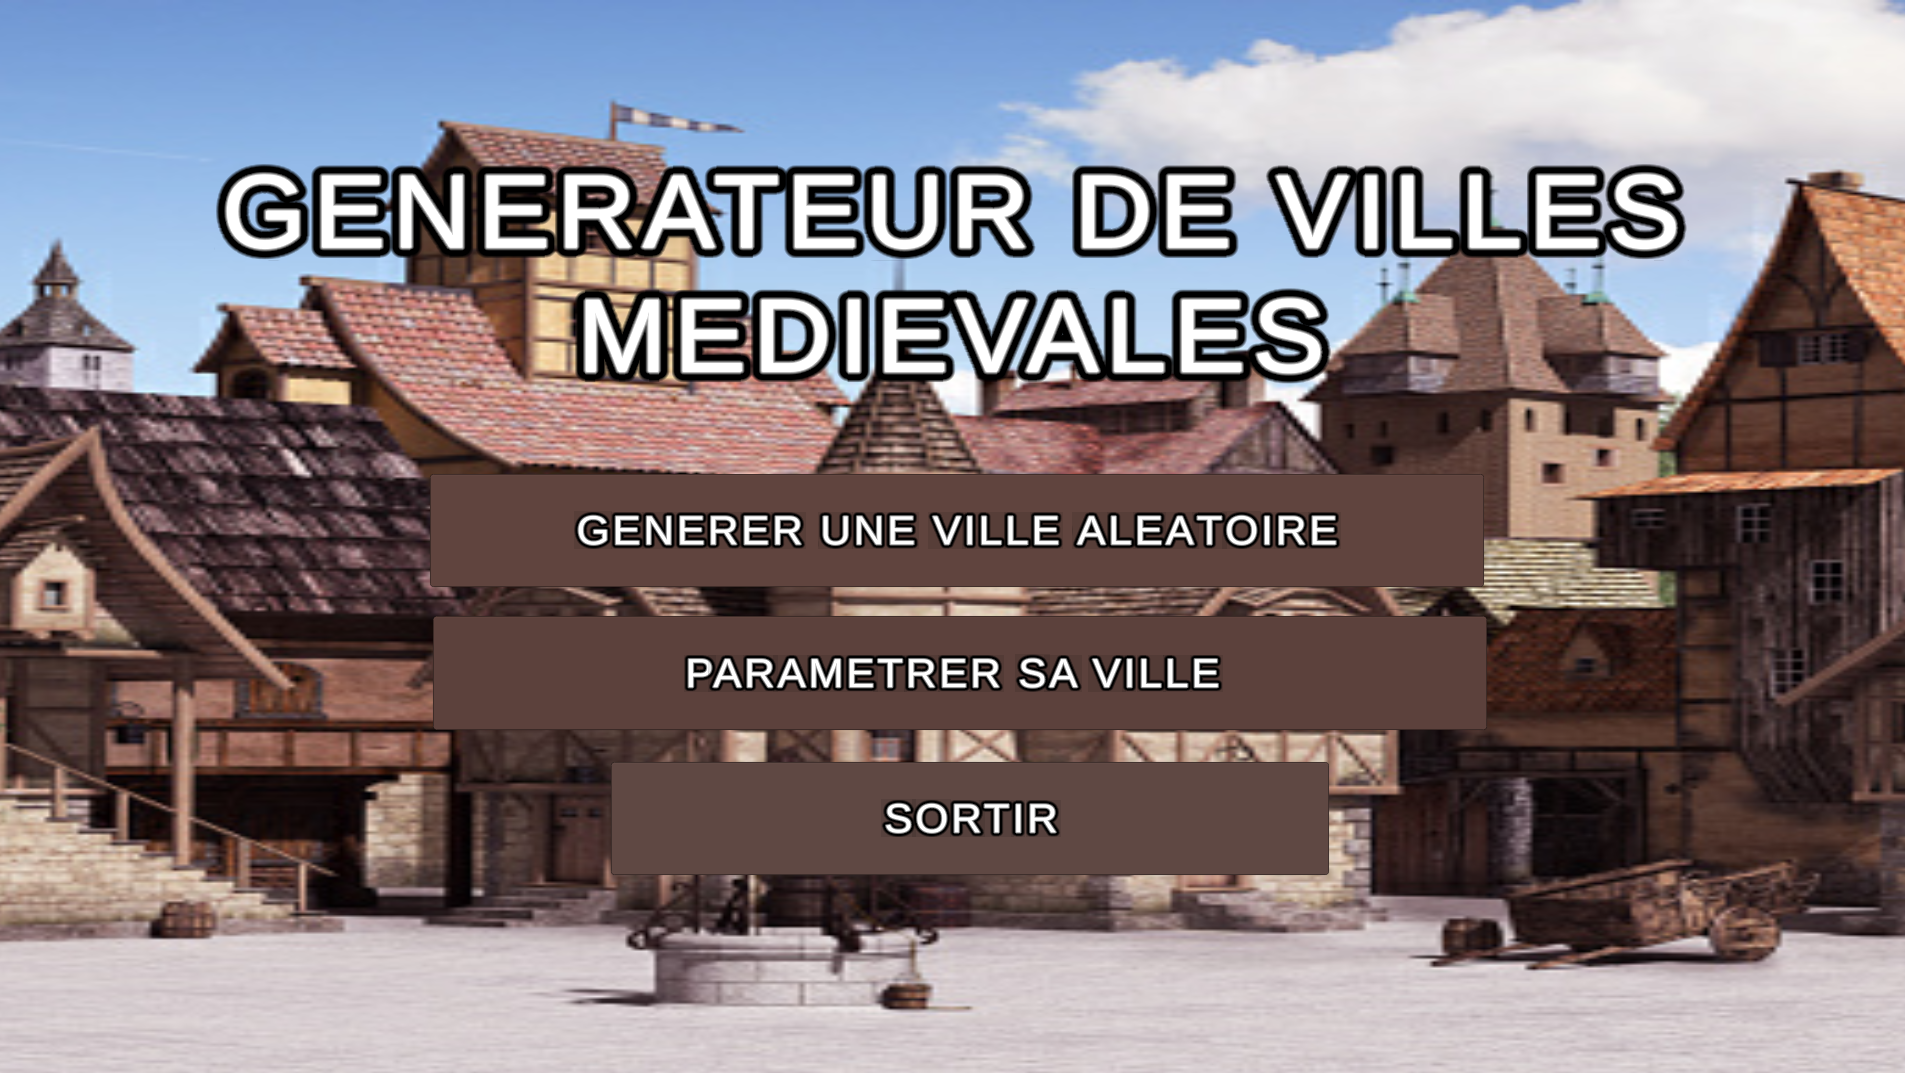
\includegraphics[height = 5 cm]{images/Interface_1.png}\\
\end{center}

Lorsque l'on décide de paramétrer la ville que l'on veut générer on a alors trois nouvelles options possibles :
\begin{itemize}
	\item gérer le type du terrain sous forme de curseur qui plus la jauge est à gauche plus le terrain est plat, plus elle est a droite plus le terrain va être en relief avec des chaînes montagneuses.
	\item gérer la taille du terrain sous forme de curseur aussi qui en fonction de  la taille choisie va influencer le nombre de routes, de bâtiments, et la taille de la muraille.
	\item décider si l'on veut une rivière sur le plan de la ville ou non.
\end{itemize}

\begin{center}
	\centering
    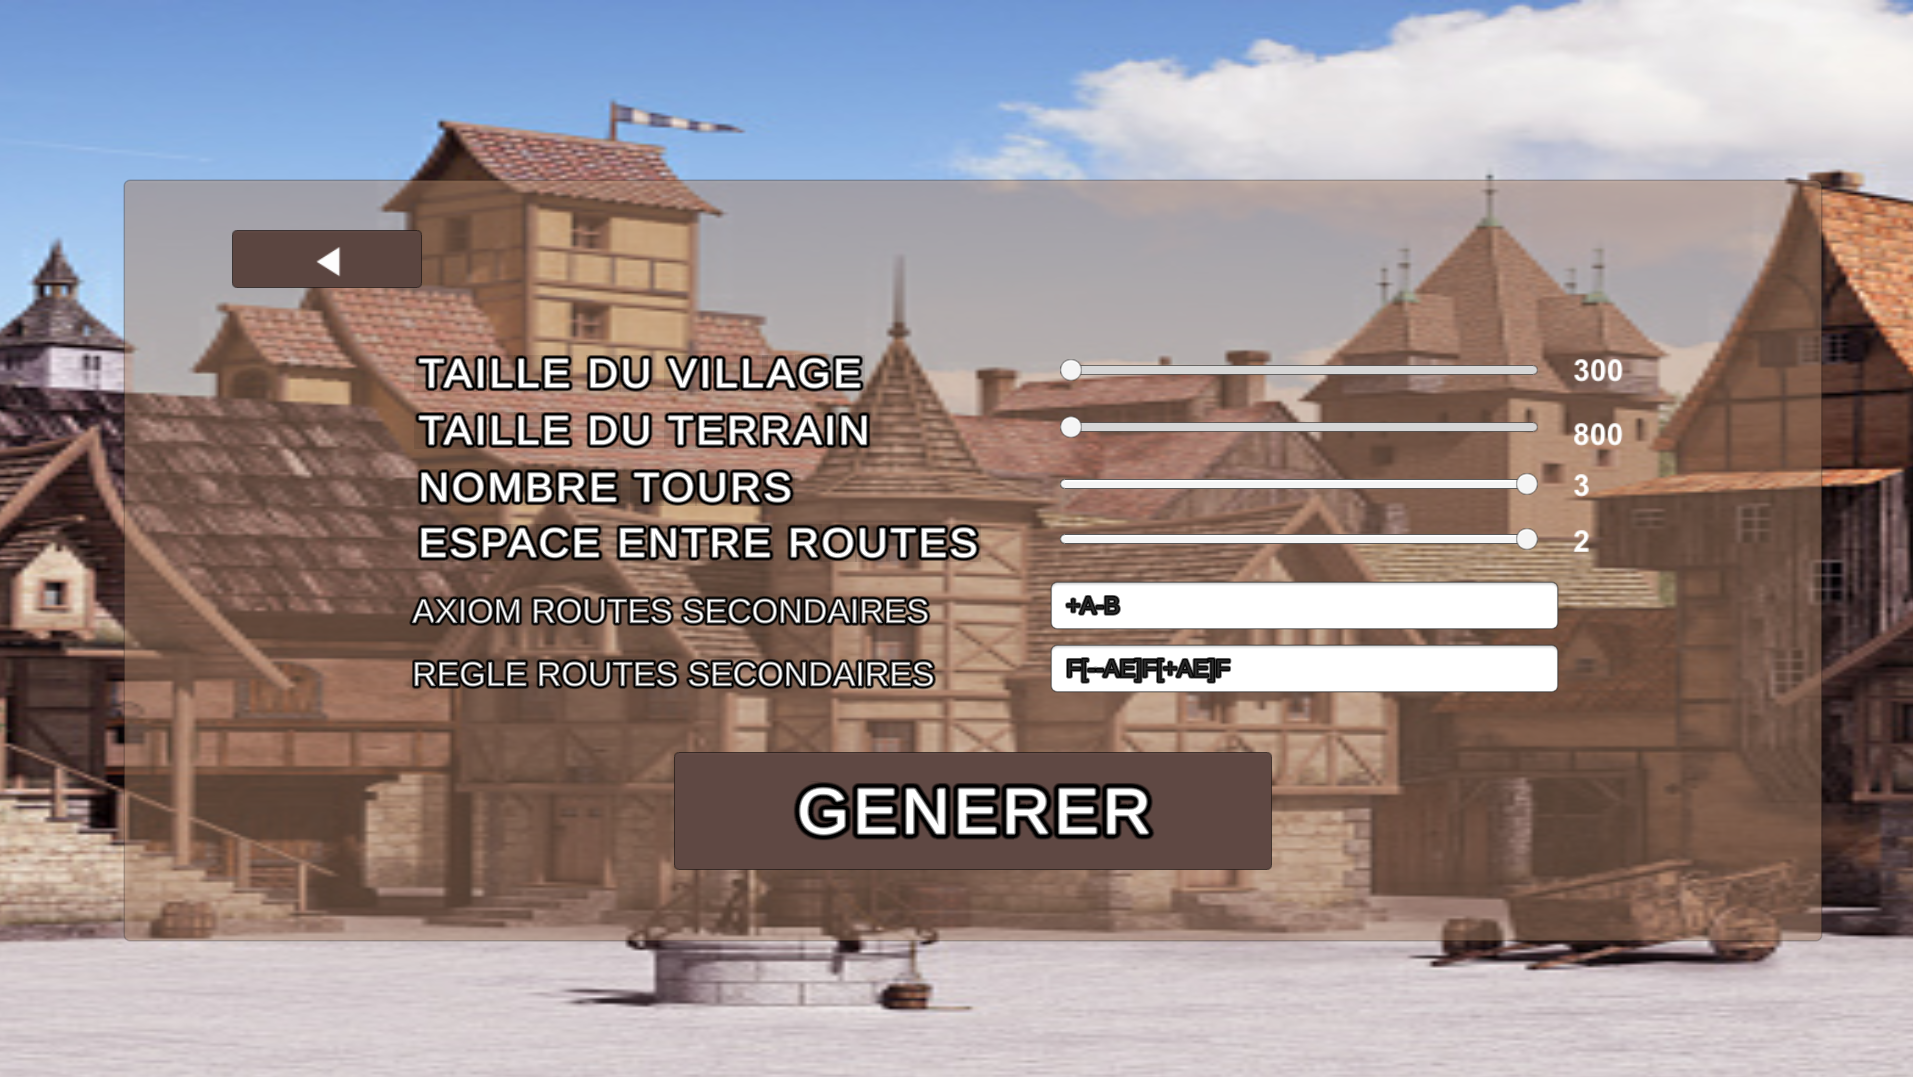
\includegraphics[height = 5 cm]{images/Interface_2.png}\\
\end{center}

En fonction des paramètres choisis, une ville sera alors générée aléatoirement et représentera un certain nombre de bâtiments placés dans des cellules avec des routes secondaires et principales apparentes, avec des éléments environnementaux comme des arbres ou des éléments un peu plus décoratifs comme des fontaines, des lampadaires ou des charettes pour rappeler le côté médiéval.

\begin{center}
	\centering
    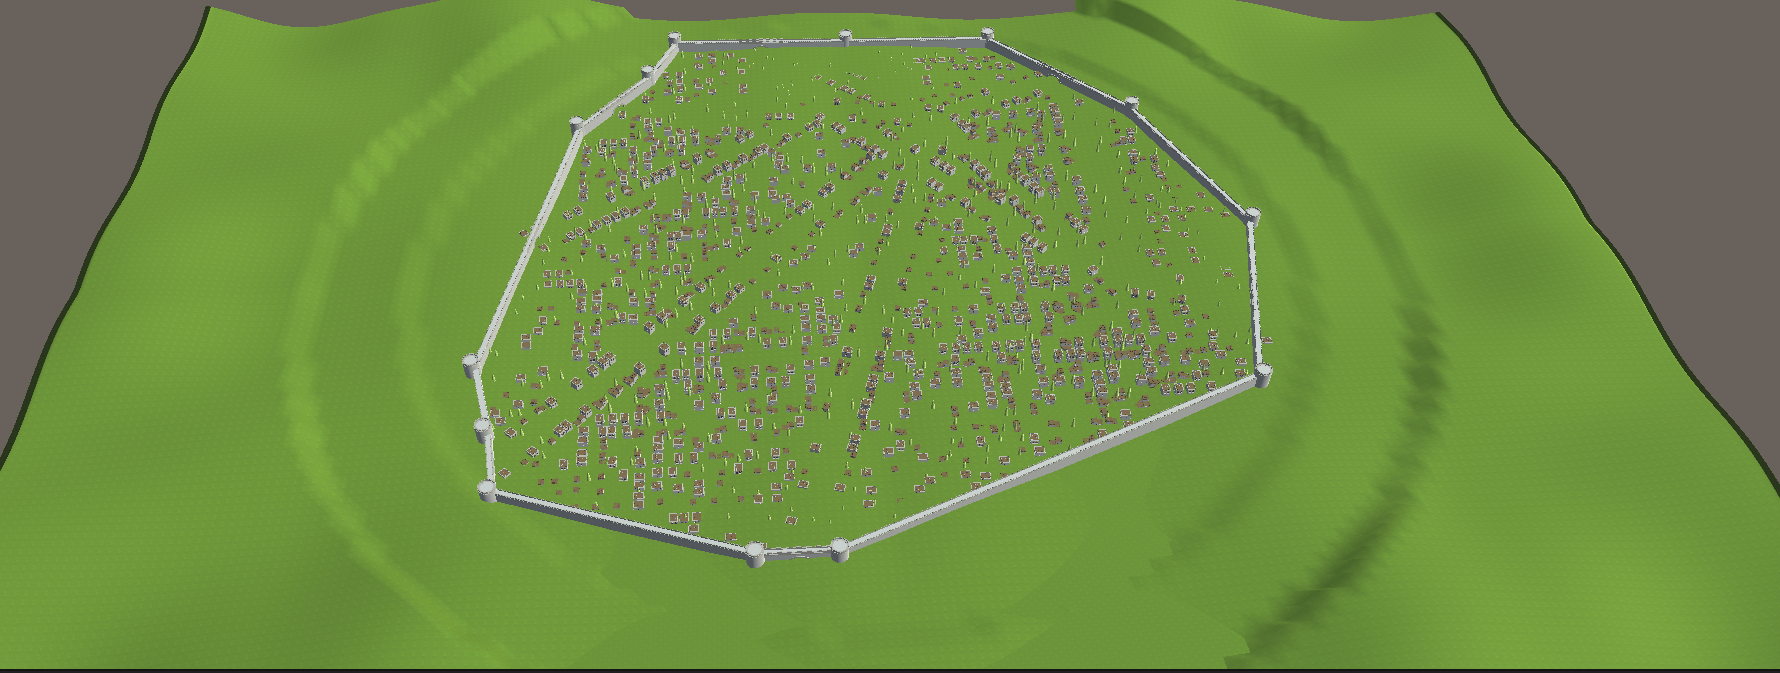
\includegraphics[height = 5 cm]{images/Ville_1.png}\\
\end{center}

La ville sera alors entourée d'une muraille pour délimiter son expansion et permettre aussi de rendre plus plat le terrain sur lequel est placé cette muraille pour ne pas avoir de contraintes de placement de ce,lule en relief à l'intérieur de la muraille.

\begin{center}
	\centering
    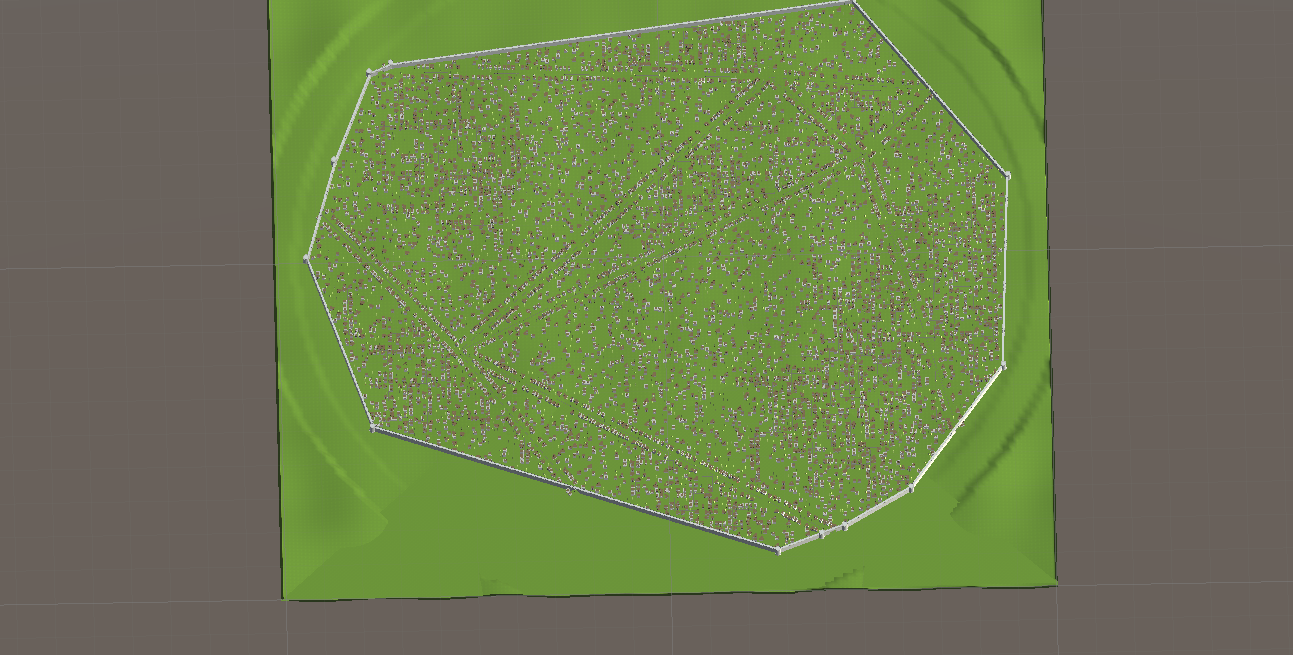
\includegraphics[height = 5 cm]{images/Ville_2.png}\\
\end{center}

L’interface a été faite avec l’outil UI sur une scène, et est donc composée de scripts en C Sharp permettant l’exécution d’une action suite à une interaction avec les différents éléments de l’interface. Lorsque l'on clique sur un bouton, c'est l'appel à la fonction C Sharp qui permet l'affichage de l'éxecution du code voulu. Les scènes en question sont numérotées et mises en place dans les paramètres de Build, ce qui permet l'affichage d'une scène de l'interface et une scène de génération de ville. 

\subsection{Génération de terrain}

La génération de terrain se fait par l'algorithme de Perlin, en théorie lorsqu'on sélectionne "Générer une ville " on affiche un terrain en relief créé par le bruit de Perlin, dans lequel la surface où se situe la ville est plane, et le contour de celle-ci est en relief, on a également des creux autour des montagnes qui représente les points d'eaux mis en place (rivières). Le relief peut être plus ou moins prononcé en fonction des coordonnées que l'on veut établir au code, plus les coordonnées seront élevées plus le bruit de Perlin sera prononcé et donc on aura un terrain avec des hautes montagnes et quasiment aucun endroit où la surface est plane (hors la ville car le code applatit la zone où on la place).

\begin{center}
	\centering
    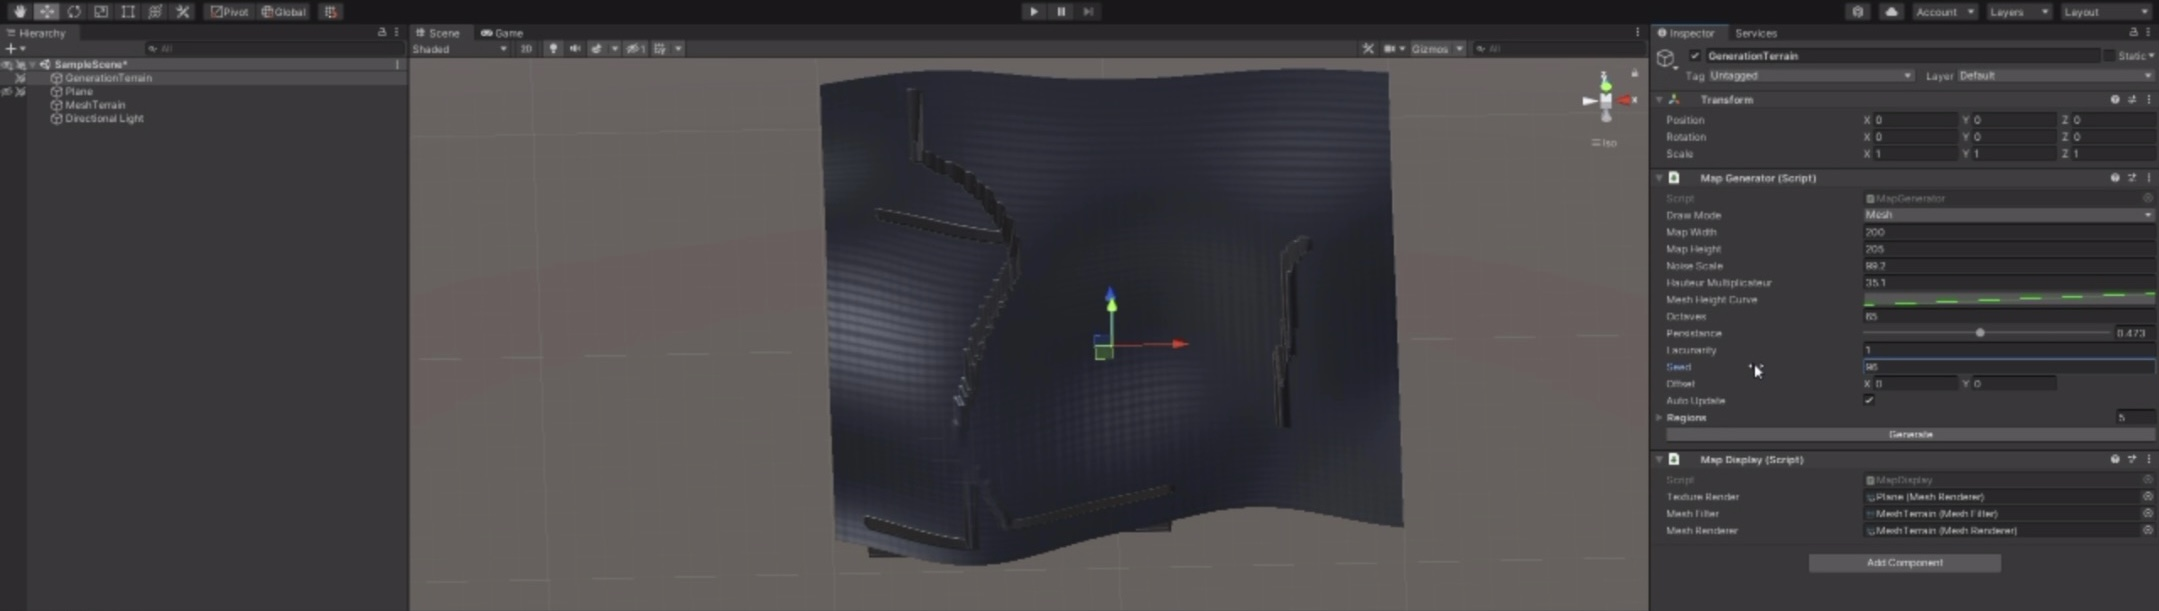
\includegraphics[height = 5 cm]{images/terrainavecriviere.jpeg}\\
\end{center}

\subsection{Génération de la ville}

La génération de la ville est aléatoire, on obtient un certain nombre de bâtiments à l'intérieur de la muraille, les bâtiments sont le plus possible placés à proximité des routes pour éviter d'avoir une génération trop aléatoire et une ville qui se rapproche le plus d'une ville urbaine, dans lequel on y retrouve des quartiers entourés par des routes secondaires, et un alignement de bâtiments autour des routes principales. Les routes sortent de la ville par des portes créées à l'intérieur de la muraille. On observe également des bâtiments à l'exterieur de la muraille mais on y reviendra dans la section bugs.

\begin{center}
	\centering
    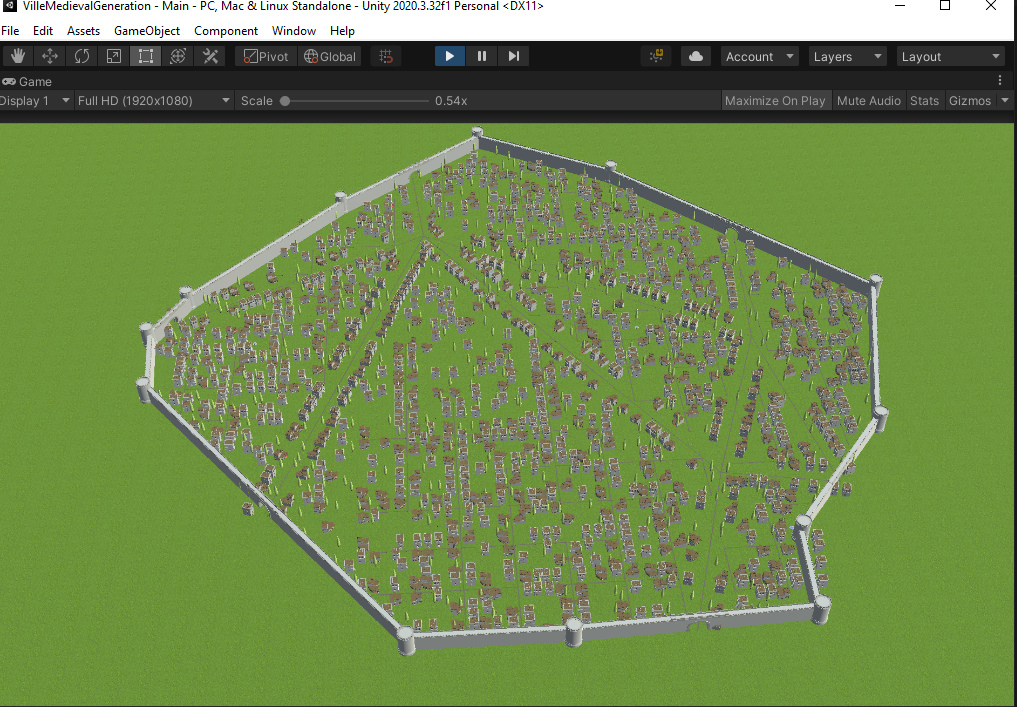
\includegraphics[height = 5 cm]{images/generationville.png}\\
\end{center}







\newpage

\section{Tests et bugs}

\subsection{Interface}

Pour la partie interface, nous avons essayé de simuler une exécution de génération de ville, en commençant par le bouton "générer une ville aléatoire" puis "paramétrer sa ville":

\begin{itemize}
	\item Générer une ville aléatoirement : Lorsqu'on appuie sur le bouton avec un ordinateur qui a la même configuration que celui utilisé pour l'analyse de l'existant, la génération de ville se fait en 10 secondes, ce qui est bien loin de ce que l'on espérait au début soit être à environ 24 000 bâtiments en 3,5 secondes comme Citygen.
	\item Paramétrer sa ville : Le bouton "paramétrer sa ville" donne accès à une nouvelle fenêtre dans laquelle il est possible de trziter la taille de la ville et si l'on veut une rivière ou non. L'affichage de la nouvelle page se fait correctement et rapidement, seulement les deux boutons affichés par la suite ne fonctionne pas, on est obligé de quitter la génération si l'on veut retourner à la page d'accueil.
\end{itemize}

\subsection{Terrain}

Pour le terrain nous avons testé les limites que celui-ci apporte, par exemple en augmentant à la limite du possible le maillage du terrain, ainsi que moduler les paramètres du bruit de Perlin pour voir si on obtient des bugs ou non.

\begin{itemize}
	\item Maillage : Lorsque l'on utilise un maillage inférieur ou égal à 250 par 250, l'affichage du terrain se fait correctement, nous n'avons pas d'erreur d'affichage et le terrain est correct.
\end{itemize}
	
\begin{center}
	\centering
    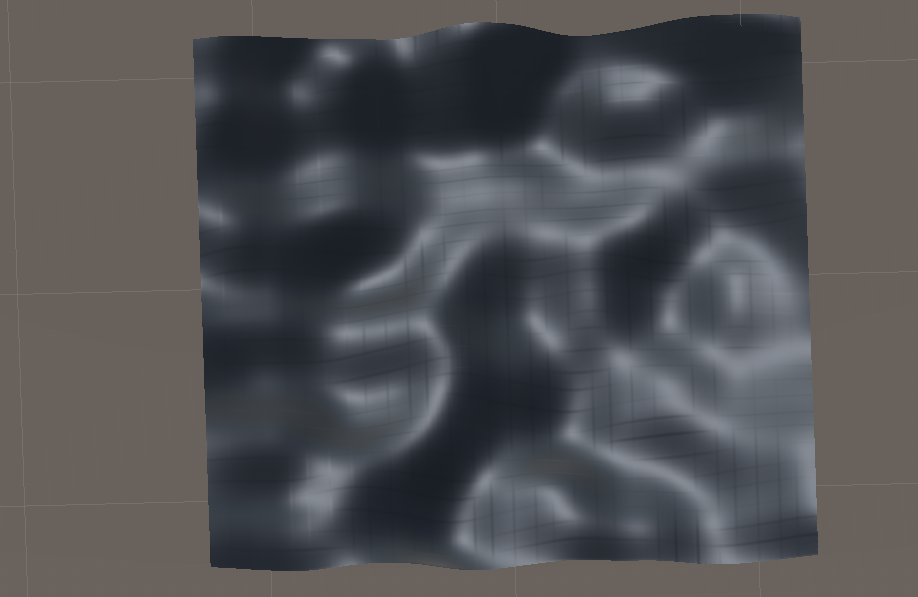
\includegraphics[height = 5 cm]{images/maille(250x250).png}\\
	 \captionof{figure}\small{Maille 250x250}
\end{center}

	Cependant lorsque l'on met en place des paramètres au-delà de cette valeur, on obtient un bruit de Perlin qui n'est pas correct car on y apperçoit des lignes, comme si la zone avait été saturée par la trop forte quantité de maillage.
	
\begin{center}
	\centering
    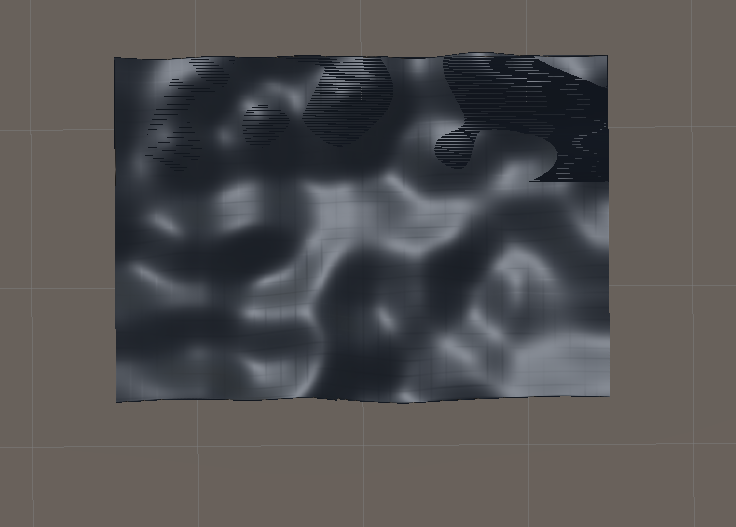
\includegraphics[height = 5 cm]{images/maille(350x350).png}\\
	 \captionof{figure}\small{Maille 350x350}
\end{center}

\begin{itemize}
	\item Bruit de Perlin : Lorsque l'on change les paramètres sur la hauteur des coordonnées et qu'on les mets à l'extrême, on obtient un terrain correct, seulement il est impossible de l'utiliser car les ondulations sont beaucoup trop conséquentes. À l'inverse si l'on met tout au minimum, on obtient un terrain plat sans bugs.
	
	\item Fusion terrain et ville : nous n'avions pas clairement réussi à fusionner le terrain et la ville lors de la génération, même si les deux éléments existe distinctement et que l'on peut mettre une ville à la main sur le terrain. Ce problème a été solutionner en mettant en place un creux sur le terrain pour mettre une partie du terrain à hauteur zéro et y placer la ville.
\end{itemize}

\subsection{Ville}

Pour tester la génération de ville nous avons mis en place un test de limite qui considère dans un premier temps le comportement d'une petite ville (citysize : 50) et celui d'une plus grande ville (citysize : 600).

\begin{itemize}
	\item Petite ville : L'exécution de la petite ville se fait assez rapidement, cependant au niveau de l'affichage on recontre quelques problèmes, les éléments de la ville sont à l'extérieur de la muraille (on observe ce phénomène également sur une plus grande ville mais moins fréquemment), il est donc impossible d'avoir une ville correcte si on veut qu'elle soit petite.
	
\begin{center}
	\centering
    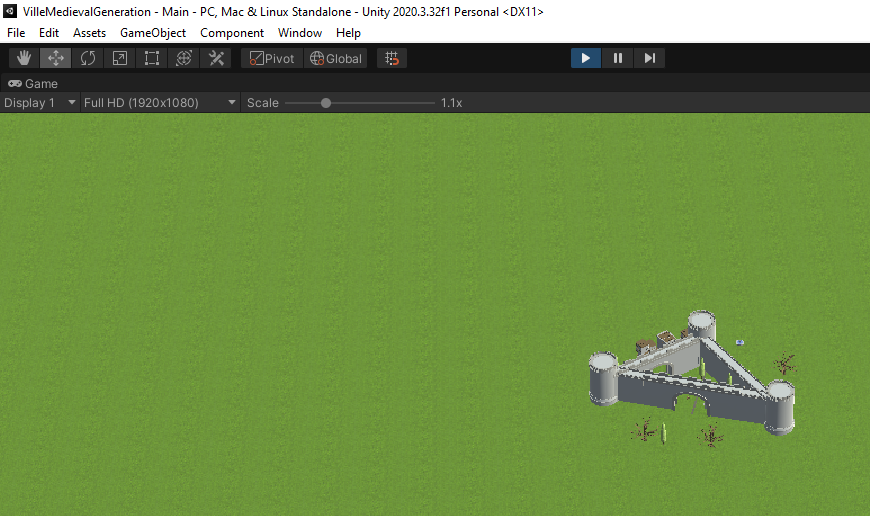
\includegraphics[height = 5 cm]{images/testville.png}\\
	\captionof{figure}\small{Ville de taille 50}
\end{center}

	\item Grande ville : L'exécution de la grande ville est un peu plus fastidieux en terme de temps et d'affichage, nous avons réussi au maximum à créer une ville de taille 600 qui met 30 secondes à se générer, au delà de cette taille l'affichage est impossible que le pc crash avant de pouvoir finir la génération. Nous remarquons que dans ce cas précis de grande ville nous n'avons pas de bug de bâtiments en dehors de la muraille, donc il est possible que le bug de la muraille dépendent de la taille de la ville.
	
\begin{center}
	\centering
    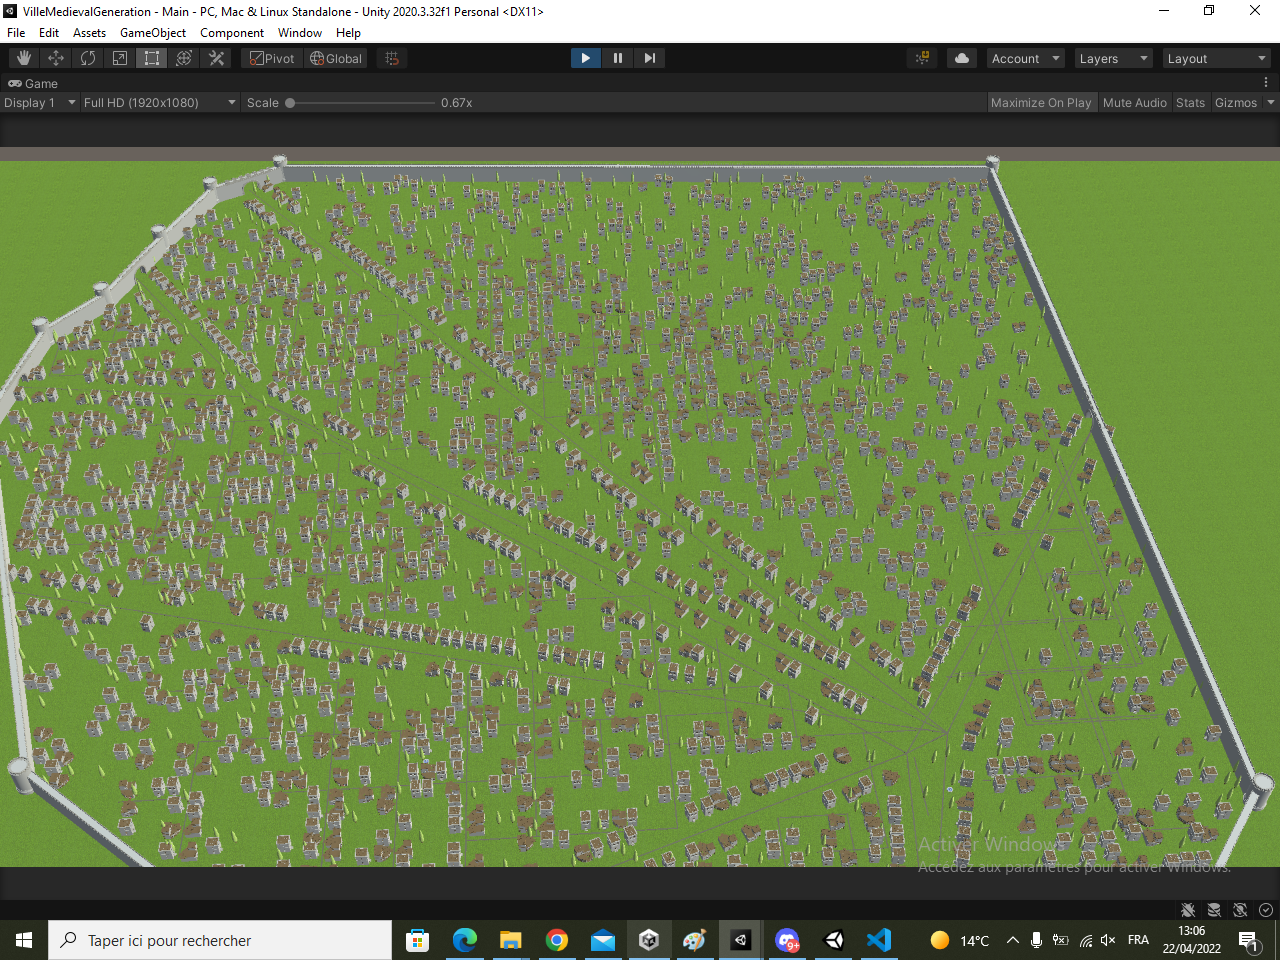
\includegraphics[height = 5 cm]{images/testville2.png}\\
	\captionof{figure}\small{Ville de taille 50}
\end{center}

	\item Ville avec terrain : il arrive aussi que la ville ne se mette pas directement en lien avec le terrain, les murailles débordent, et le bug sur les bâtiments qui dépassent de la muraille est aussi fréquent. 
	
	
\begin{center}
	\centering
    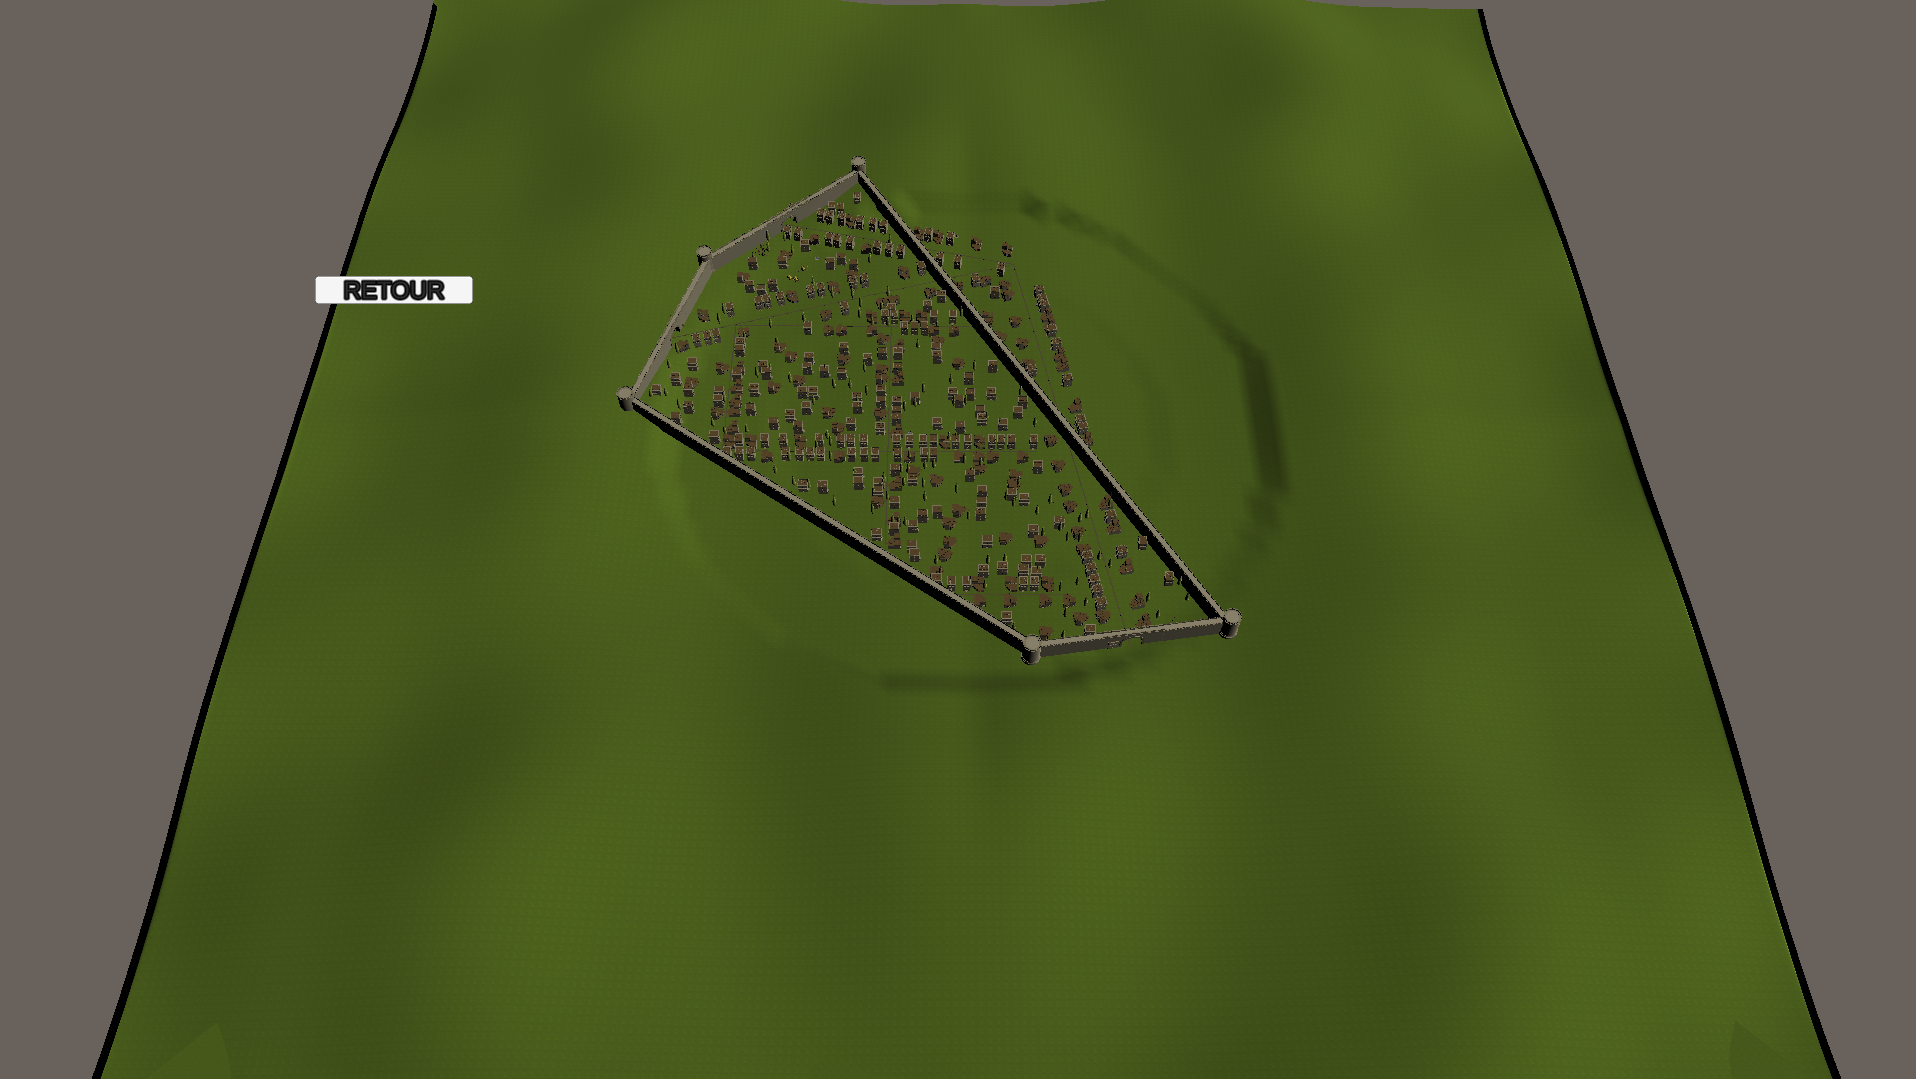
\includegraphics[height = 5 cm]{images/testville3.png}\\
	\captionof{figure}\small{Ville avec terrain}
\end{center}
	
\end{itemize}

Nous avions également rencontré des bugs sur la générations des terrains qui ne se faisait pas autour des routes mais nous avons solutionner le problème, également sur les L-system qui ont créé des routes similaires à la création de plusieurs branches qui se croisaient, nous avons réglé le problème en créant des routes qui sont plus rectangulaires. Également si nous mettons en place plusieurs routes principales, nous ne recontrons pas de bug (à la limite du lisible) et chaque route principales sort par une porte de la muraille.

\section{A finir}

Nous n'avons pas réussi à mettre en place plusieurs éléments que nous aurions aimé pouvoir régler avant le rendu, les voici :

\begin{itemize}
	\item Créer des rivières à l'intérieur de la ville
	\item Faire évoluer la ville en une ville moderne
	\item Régler l'interface pour pouvoir choisir la taille de la ville
	\item Rendre les routes plus visibles avec une texture
	\item Sauvegarder le résultat obtenu
\end{itemize}

\section{Conclusion}

Pour conclure ce projet de génération de ville aléatoire, nous sommes plutôt satisfaits de ce que nous avons produit même si il manque encore beaucoup de détails que nous aurions aimé implémenter. Les besoins principaux ont été remplis, cependant nous estimons avoir été trop optimistes sur la quantité de besoins à mettre en place car nous ne nous étions pas rendu compte au premiers aborts de la quantité de travail que cela représentait.

Nous tenions à remercier notre chargé de TD, Monsieur Philippe Narbel qui nous a accompagné tout le long de la rédaction de ce mémoire et du code, et qui nous a été d'une aide précieuse.



\newpage

\bibliography{sources.bib}

\end{document}

